\documentclass[slidestop,compress,mathserif]{beamer}

%%% To get handouts:
%\documentclass[11pt,containsverbatim,handout]{beamer}
%% include when making handouts
%\usepackage{pgfpages}
%\pgfpagesuselayout{4 on 1}[letterpaper,landscape,border shrink=5mm]

%%% To get rid of solutions on handouts:
\newcommand{\soln}[1]{\textit{#1}}				% For slides
%\newcommand{\soln}[1]{ }	% For handouts

\newcommand{\solnGr}[1]{#1}
%\newcommand{\solnGr}{ }

\usetheme{metropolis}

%%%%%%%%%%%%%%%%
% Packages
%%%%%%%%%%%%%%%%

\usepackage{geometry}
\usepackage{graphicx}
\usepackage{amssymb}
%\usepackage{cancel}
\usepackage{epstopdf}
\usepackage{amsmath}  	% this permits text in eqnarray among other benefits
\usepackage{url}		% produces hyperlinks
\usepackage{hyperref}	% allows for color usage in tables
\usepackage[english]{babel}
\usepackage[latin1]{inputenc}
\usepackage{colortbl}	% allows for color usage in tables
\usepackage{multirow}	% allows for rows that span multiple rows in tables
\usepackage{color}		% this package has a variety of color options
\usepackage{pgf}
\usepackage{calc}
\usepackage{ulem}
\usepackage{multicol}
\usepackage{textcomp}
\usepackage{txfonts}
\usepackage{listings}
\usepackage{tikz}
\usepackage{array}
\usepackage{wasysym}
\usepackage{fancyvrb}


%%%%%%%%%%%%%%%%
% Remove navigation symbols
%%%%%%%%%%%%%%%%

\setbeamertemplate{navigation symbols}{}

%%%%%%%%%%%%%%%%
% User defined colors
%%%%%%%%%%%%%%%%

\xdefinecolor{oiB}{rgb}{0.22,0.52,0.72}
\definecolor{oiG}{rgb}{.298,.447,.114}
\xdefinecolor{hlblue}{rgb}{0.051,0.65,1}
\xdefinecolor{gray}{rgb}{0.5, 0.5, 0.5}
\xdefinecolor{darkGray}{rgb}{0.3, 0.3, 0.3}
\xdefinecolor{darkerGray}{rgb}{0.2, 0.2, 0.2}
\xdefinecolor{rubineRed}{rgb}{0.89,0,0.30}
\xdefinecolor{irishGreen}{rgb}{0,0.60,0}	
\definecolor{lightGreen}{rgb}{0.387,0.581,0.148} 

%%%%%%%%%%%%%%%%
% Template colors
%%%%%%%%%%%%%%%%

%\setbeamercolor*{palette primary}{fg=white,bg= oiB!80!black!90}
%\setbeamercolor*{palette secondary}{fg=black,bg= oiB!80!black}
%\setbeamercolor*{palette tertiary}{fg=white,bg= oiB!80!black!80}
%\setbeamercolor*{palette quaternary}{fg=white,bg= oiB}
%\setbeamercolor{structure}{fg= oiB}
%\setbeamercolor{frametitle}{bg= oiB!90}
%\setbeamertemplate{blocks}[shadow=false]
%\setbeamersize{text margin left=2em,text margin right=2em}

%\setbeamercolor{code body}{bg=gray!20!white!80,fg=black}


%%%%%%%%%%%%%%%%
% Get rid of fancy enumerated list bullets
%%%%%%%%%%%%%%%%

%\setbeamertemplate{enumerate items}[default]

%%%%%%%%%%%%%%%%
% Custom commands
%%%%%%%%%%%%%%%%

% degree
\newcommand{\degree}{\ensuremath{^\circ}}

% cite
\newcommand{\ct}[1]{
\vfill
{\tiny #1}}

% Note
\newcommand{\Note}[1]{
\rule{2.5cm}{0.25pt} \\ \textit{\footnotesize{\textcolor{rubineRed}{Note:} \textcolor{darkerGray}{#1}}}}

% Remember
\newcommand{\Remember}[1]{\textit{\scriptsize{\textcolor{orange}{Remember:} #1}}}

% expected counts
\newcommand{\ex}[1]{\textit{\textcolor{blue}{#1}}}

% red
\newcommand{\red}[1]{\textit{\textcolor{rubineRed}{#1}}}

% pink
\newcommand{\pink}[1]{\textit{\textcolor{rubineRed!90!white!50}{#1}}}

% green
\newcommand{\green}[1]{\textit{\textcolor{irishGreen}{#1}}}

% orange
\newcommand{\orange}[1]{\textit{\textcolor{orange}{#1}}}

% links: webURL, webLin, appLink
\newcommand{\webURL}[1]{\urlstyle{same}{ \textit{\textcolor{darkGray}{\url{#1}}}}}
\newcommand{\webLink}[2]{\href{#1}{\textcolor{darkGray}{{#2}}}}
\newcommand{\appLink}[2]{\href{#1}{\textcolor{white}{{#2}}}}

% mail
\newcommand{\mail}[1]{\href{mailto:#1}{\textit{\textcolor{darkGray}{#1}}}}

% highlighting: hl, hlGr, mathhl
\newcommand{\hl}[1]{\textit{\textcolor{hlblue}{#1}}}
\newcommand{\hlGr}[1]{\textit{\textcolor{lightGreen}{#1}}}
\newcommand{\mathhl}[1]{\textcolor{hlblue}{\ensuremath{#1}}}

% two col: two columns
\newenvironment{twocol}[4]{
\begin{columns}[c]
\column{#1\textwidth}
#3
\column{#2\textwidth}
#4
\end{columns}
}

% slot (for probability calculations)
\newenvironment{slot}[2]{
\begin{array}{c} 
\underline{#1} \\ 
#2
\end{array}
}

% pr: left and right parentheses
\newcommand{\pr}[1]{
\left( #1 \right)
}

% solnMult: solutions for practice questions

\newcommand{\solnMult}[1]{
\item[] \vspace{-0.59cm}
\only<1>{\item #1}
\soln{\only<2->{\item \orange{#1}}}
}

% cancel
\newcommand{\cancel}[1]{%
    \tikz[baseline=(tocancel.base)]{
        \node[inner sep=0pt,outer sep=0pt] (tocancel) {#1};
        \draw[red, line width=0.5mm] (tocancel.south west) -- (tocancel.north east);
    }%
}

% removepagenumbers
\newcommand{\removepagenumbers}{% 
  \setbeamertemplate{footline}{}
}

%%%%%%%%%%%%%%%%
% Custom boxes
%%%%%%%%%%%%%%%%

% app: application exercise

\setbeamercolor{app body}{fg=oiG}

\newcommand{\app}[1]{
\begin{beamerboxesrounded}[shadow = false, lower = app body]{}
#1
\end{beamerboxesrounded}
}

% dq: discussion question

\setbeamercolor{disc ques body}{fg=oiB}

\newcommand{\dq}[1]{
\begin{beamerboxesrounded}[shadow = false, lower = disc ques body]{}
#1
\end{beamerboxesrounded}
}

% pq: practice question

\setbeamercolor{prac ques body}{fg=oiB}

\newcommand{\pq}[1]{
\begin{beamerboxesrounded}[shadow = false, lower = prac ques body]{}
#1
\end{beamerboxesrounded}
}

% formula

\setbeamercolor{formula body}{fg=oiB!55!black!95}

\newcommand{\formula}[1]{
\begin{beamerboxesrounded}[shadow = false, lower = formula body]{}
#1
\end{beamerboxesrounded}
}


%%%%%%%%%%%%%%%%
% Change margin
%%%%%%%%%%%%%%%%

\newenvironment{changemargin}[2]{%
\begin{list}{}{%
\setlength{\topsep}{0pt}%
\setlength{\leftmargin}{#1}%
\setlength{\rightmargin}{#2}%
\setlength{\listparindent}{\parindent}%
\setlength{\itemindent}{\parindent}%
\setlength{\parsep}{\parskip}%
}%
\item}{\end{list}}

%%%%%%%%%%%%%%%%
% Footnote
%%%%%%%%%%%%%%%%

\long\def\symbolfootnote[#1]#2{\begingroup%
\def\thefootnote{\fnsymbol{footnote}}\footnote[#1]{#2}\endgroup}

%%%%%%%%%%%%%%%%
% Commands from the book
%%%%%%%%%%%%%%%%

\newenvironment{data}[1]{\texttt{#1}}{}
\newenvironment{var}[1]{\texttt{#1}}{}
\newenvironment{resp}[1]{\texttt{#1}}{}

%%%%%%%%%%%%%%%%
% Graphics
%%%%%%%%%%%%%%%%

\DeclareGraphicsRule{.tif}{png}{.png}{`convert #1 `dirname #1`/`basename #1 .tif`.png}

%%%%%%%%%%%%%%%%%%%%%

\title[Chp 3: Distributions of RVs]{Chapter 3: Distributions of Random Variables}
\author{OpenIntro Statistics, 2nd Edition}
\date{}
\institute{}

%%%%%%%%%%%%%%%%%%%%%

\begin{document}

%%%%%%%%%%%%%%%%%%%%%

% Title Page

\begin{frame}[plain]

\titlepage

{\footnotesize Slides developed by Mine \c{C}etinkaya-Rundel of OpenIntro \\
The slides may be copied, edited, and/or shared via the \webLink{http://creativecommons.org/licenses/by-sa/3.0/us/}{CC BY-SA license} \\
Some images may be included under fair use guidelines (educational purposes)}

\end{frame}

%%%%%%%%%%%%%%%%%%%%%%%%%%%%%%%%%%%%

\section{Normal distribution}

%%%%%%%%%%%%%%%%%%%%%%%%%%%%%%%%%%%%

\begin{frame}
\frametitle{Normal distribution}

\begin{itemize}

\item Unimodal and symmetric, bell shaped curve

\item Many variables are nearly normal, but none are exactly normal

\item Denoted as \mathhl{N(\mu,\sigma)} $\rightarrow$ Normal with mean $\mu$ and standard deviation $\sigma$

\end{itemize}

\begin{center}
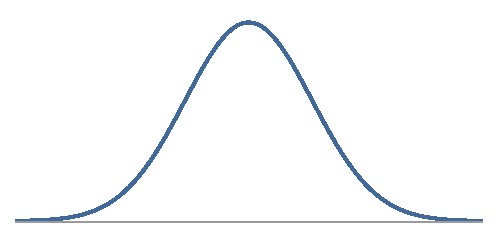
\includegraphics[width=0.7\textwidth]{3-1_normal_distribution/figures/simpleNormal/simpleNormal}
\end{center}

\end{frame}

%%%%%%%%%%%%%%%%%%%%%%%%%%%%%%%%%%%%

\begin{frame}
\frametitle{Heights of males}

\twocol{0.5}{0.5}{
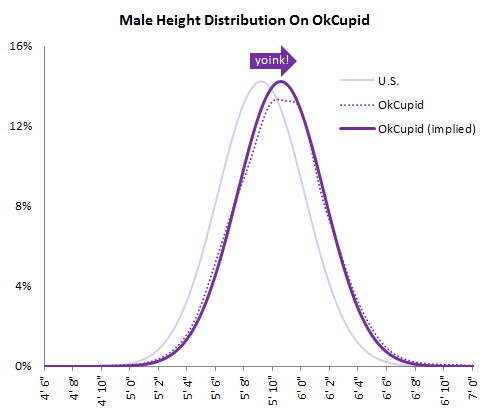
\includegraphics[width=\textwidth]{3-1_normal_distribution/figures/ok_cupid/ok_cupid_men} \\
}
{
\pause
{\footnotesize``The male heights on OkCupid very nearly follow the expected normal distribution -- except the whole thing is shifted to the right of where it should be. Almost universally guys like to add a couple inches." 

``You can also see a more subtle vanity at work: starting at roughly 5' 8", the top of the dotted curve tilts even further rightward. This means that guys as they get closer to six feet round up a bit more than usual, stretching for that coveted psychological benchmark."
}
}

\ct{\webURL{http://blog.okcupid.com/index.php/the-biggest-lies-in-online-dating/}}

\end{frame}

%%%%%%%%%%%%%%%%%%%%%%%%%%%%%%%%%%%%

\begin{frame}
\frametitle{Heights of females}

\twocol{0.5}{0.5}{
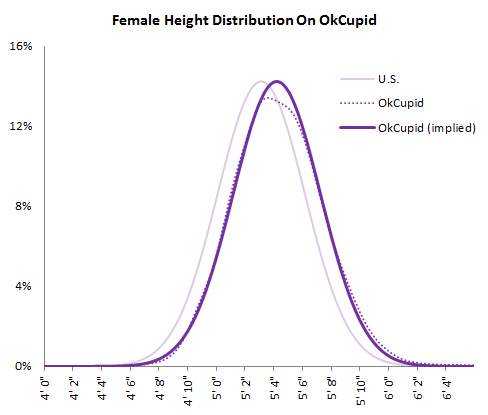
\includegraphics[width=\textwidth]{3-1_normal_distribution/figures/ok_cupid/ok_cupid_women} \\
}
{
\pause
{\footnotesize ``When we looked into the data for women, we were surprised to see height exaggeration was just as widespread, though without the lurch towards a benchmark height."
}
}

\vfill

\ct{\webURL{http://blog.okcupid.com/index.php/the-biggest-lies-in-online-dating/}}

\end{frame}

%%%%%%%%%%%%%%%%%%%%%%%%%%%%%%%%%%%%

\subsection{Normal distribution model}

%%%%%%%%%%%%%%%%%%%%%%%%%%%%%%%%%%%%

\begin{frame}
\frametitle{Normal distributions with different parameters}

\vspace{-0.5cm}
\begin{center}
$\mu$: mean, $\sigma$: standard deviation
\[N(\mu = 0, \sigma = 1) \hspace{1.4cm} N(\mu = 19, \sigma = 4) \]
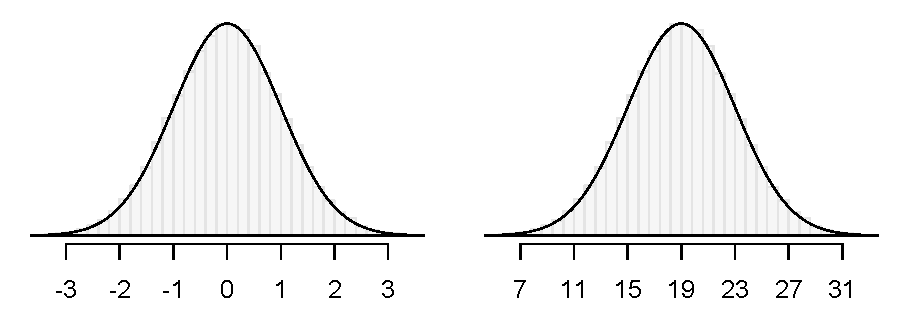
\includegraphics[width=0.6\textwidth]{3-1_normal_distribution/figures/twoSampleNormals/twoSampleNormals} \\
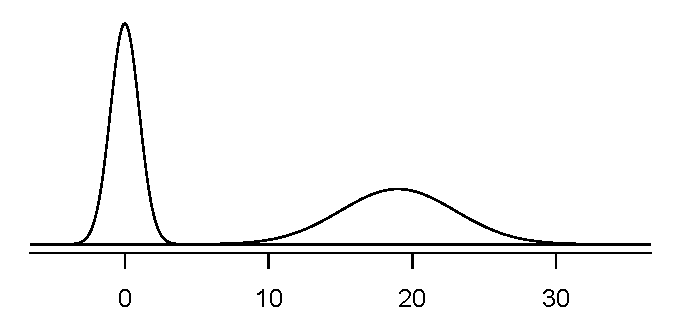
\includegraphics[width=0.6\textwidth]{3-1_normal_distribution/figures/twoSampleNormalsStacked/twoSampleNormalsStacked}
\end{center}

\end{frame}

%%%%%%%%%%%%%%%%%%%%%%%%%%%%%%%%%%%%

\subsection{Standardizing with Z scores}

%%%%%%%%%%%%%%%%%%%%%%%%%%%%%%%%%%%%

\begin{frame}
\frametitle{}

\dq{SAT scores are distributed nearly normally with mean 1500 and standard deviation 300. ACT scores are distributed nearly normally with mean 21 and standard deviation 5. A college admissions officer wants to determine which of the two applicants scored better on their standardized test with respect to the other test takers: Pam, who earned an 1800 on her SAT, or Jim, who scored a 24 on his ACT?}

\begin{center}
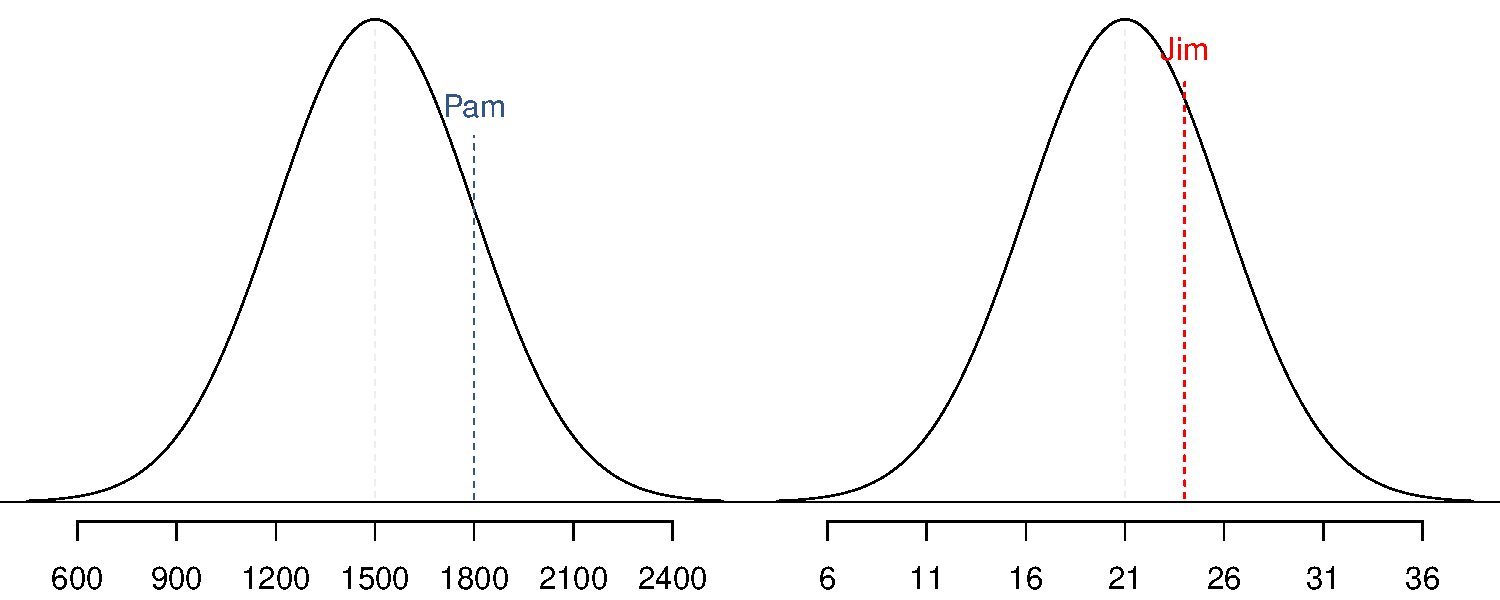
\includegraphics[width=\textwidth]{3-1_normal_distribution/figures/satActNormals/satActNormals}
\end{center}

\end{frame}

%%%%%%%%%%%%%%%%%%%%%%%%%%%%%%%%%%%%

\begin{frame}
\frametitle{Standardizing with Z scores}

Since we cannot just compare these two raw scores, we instead compare how many standard deviations beyond the mean each observation is.

\begin{itemize}

\item Pam's score is $\frac{1800 - 1500}{300} = 1$ standard deviation above the mean.

\item Jim's score is $\frac{24 - 21}{5} = 0.6$ standard deviations above the mean.

\end{itemize}

\begin{center}
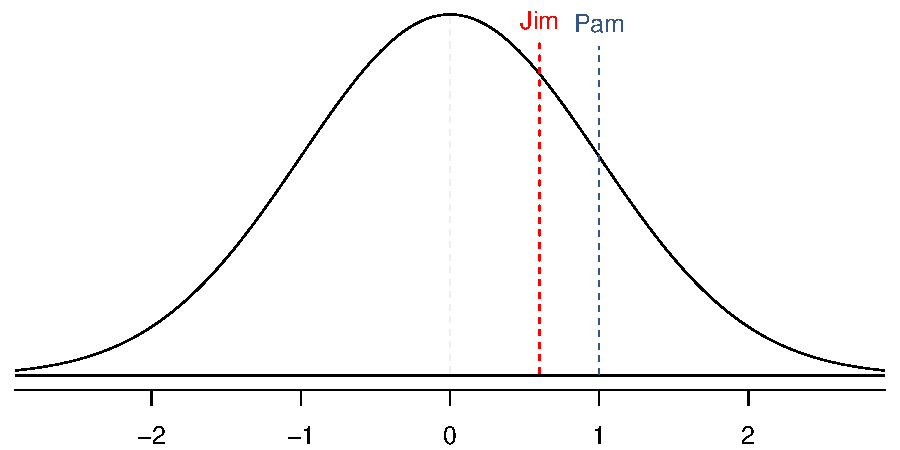
\includegraphics[width=0.7\textwidth]{3-1_normal_distribution/figures/satActNormals/satActNormalsStandardized}
\end{center}

\end{frame}

%%%%%%%%%%%%%%%%%%%%%%%%%%%%%%%%%%%%

\begin{frame}
\frametitle{Standardizing with Z scores (cont.)}

\begin{itemize}

\item These are called \hl{standardized} scores, or \hl{Z scores}.

\item Z score of an observation is the number of standard deviations it falls above or below the mean.
\formula{\[Z = \frac{observation - mean}{SD}\]}

\item Z scores are defined for distributions of any shape, but only when the distribution is normal can we use Z scores to calculate percentiles.

\item Observations that are more than 2 SD away from the mean ($|Z| > 2$) are usually considered unusual.

\end{itemize}

\end{frame}

%%%%%%%%%%%%%%%%%%%%%%%%%%%%%%%%%%%%

\begin{frame}
\frametitle{Percentiles}

\begin{itemize}

\item \hl{Percentile} is the percentage of observations that fall below a given data point. 

\item Graphically, percentile is the area below the probability distribution curve to the left of that observation.

\end{itemize}

\begin{center}
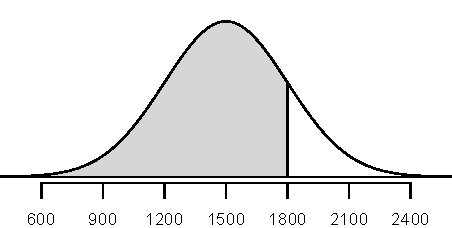
\includegraphics[width=0.7\textwidth]{3-1_normal_distribution/figures/satBelow1800/satBelow1800}
\end{center}

\end{frame}

%%%%%%%%%%%%%%%%%%%%%%%%%%%%%%%%%%%%

%\begin{frame}
%\frametitle{}
%
%\dq{Approximately what percent of students score below 1800 on the SAT? (Hint: Use the 68-95-99.7\% rule.)}
%
%\only<1>{
%\begin{center}
%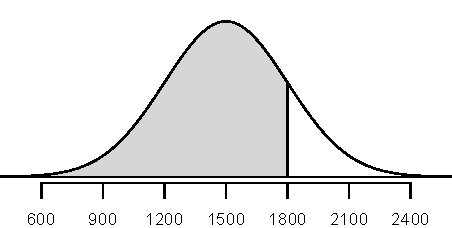
\includegraphics[width=0.7\textwidth]{3-1_normal_distribution/figures/satBelow1800/satBelow1800}
%\end{center}
%}
%
%\only<2 | handout:0>{
%\begin{center}
%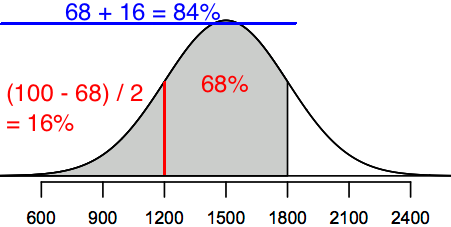
\includegraphics[width=0.7\textwidth]{3-1_normal_distribution/figures/satBelow1800/satBelow1800_soln}
%\end{center}
%}
%
%\soln{\only<2>{
%\begin{align*}
%100 - 68 &= 32\% \\
%32 / 2 &= 16\% \\
%68 + 16 &= 84\%
%\end{align*}}}
%
%\end{frame}
%
%%%%%%%%%%%%%%%%%%%%%%%%%%%%%%%%%%%%%

\subsection{Normal probability table}

%%%%%%%%%%%%%%%%%%%%%%%%%%%%%%%%%%%%

\begin{frame}[fragile]
\frametitle{Calculating percentiles - using computation}

There are many ways to compute percentiles/areas under the curve:

\begin{itemize}
\item R:
\end{itemize}
\begin{beamerboxesrounded}[shadow = false, lower = code body]{}
{\small \begin{verbatim}
> pnorm(1800, mean = 1500, sd = 300)
[1] 0.8413447
\end{verbatim}
}
\end{beamerboxesrounded}
\begin{itemize}
\item Applet: {\small \webURL{http://www.socr.ucla.edu/htmls/SOCR_Distributions.html}}
\begin{center}
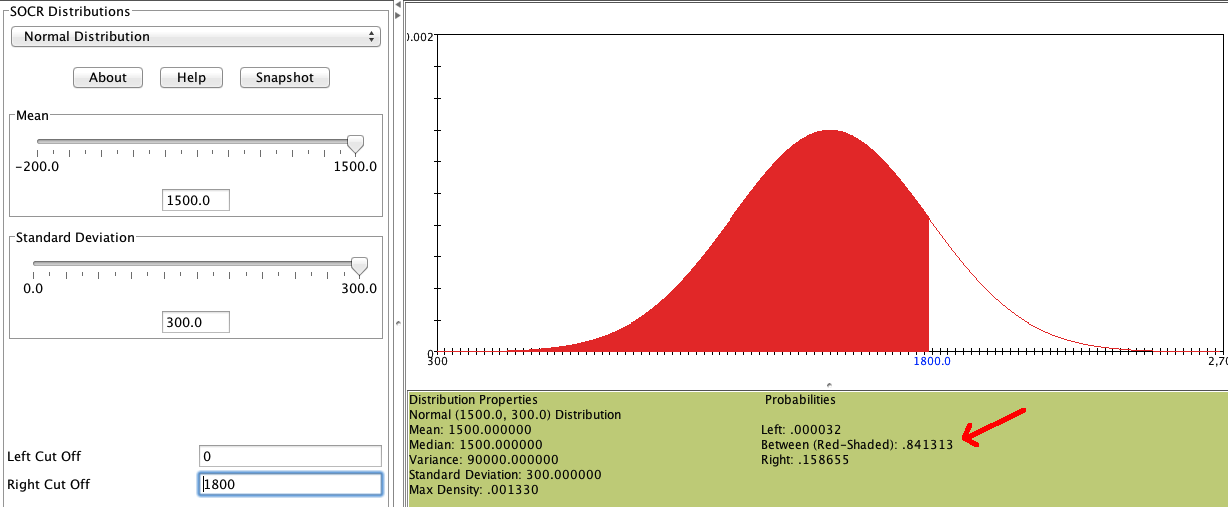
\includegraphics[width=0.8\textwidth]{3-1_normal_distribution/figures/applet}
\end{center}

\end{itemize}


\end{frame}

%%%%%%%%%%%%%%%%%%%%%%%%%%%%%%%%%%%%

\begin{frame}[fragile]
\frametitle{Calculating percentiles - using tables}

{\footnotesize
\begin{tabular}{c | >{\columncolor[gray]{0.6}[0pt]}rrrrr | rrrrr |}
  \cline{2-11}
&&&& \multicolumn{4}{c}{Second decimal place of $Z$} &&& \\
  \cline{2-11}
$Z$ & 0.00 & 0.01 & 0.02 & 0.03 & 0.04 & 0.05 & 0.06 & 0.07 & 0.08 & 0.09 \\
  \hline
  \hline
0.0 & \tiny{0.5000} & \tiny{0.5040} & \tiny{0.5080} & \tiny{0.5120} & \tiny{0.5160} & \tiny{0.5199} & \tiny{0.5239} & \tiny{0.5279} & \tiny{0.5319} & \tiny{0.5359} \\
  0.1 & \tiny{0.5398} & \tiny{0.5438} & \tiny{0.5478} & \tiny{0.5517} & \tiny{0.5557} & \tiny{0.5596} & \tiny{0.5636} & \tiny{0.5675} & \tiny{0.5714} & \tiny{0.5753} \\
  0.2 & \tiny{0.5793} & \tiny{0.5832} & \tiny{0.5871} & \tiny{0.5910} & \tiny{0.5948} & \tiny{0.5987} & \tiny{0.6026} & \tiny{0.6064} & \tiny{0.6103} & \tiny{0.6141} \\
  0.3 & \tiny{0.6179} & \tiny{0.6217} & \tiny{0.6255} & \tiny{0.6293} & \tiny{0.6331} & \tiny{0.6368} & \tiny{0.6406} & \tiny{0.6443} & \tiny{0.6480} & \tiny{0.6517} \\
  0.4 & \tiny{0.6554} & \tiny{0.6591} & \tiny{0.6628} & \tiny{0.6664} & \tiny{0.6700} & \tiny{0.6736} & \tiny{0.6772} & \tiny{0.6808} & \tiny{0.6844} & \tiny{0.6879} \\
  \hline
  0.5 & \tiny{0.6915} & \tiny{0.6950} & \tiny{0.6985} & \tiny{0.7019} & \tiny{0.7054} & \tiny{0.7088} & \tiny{0.7123} & \tiny{0.7157} & \tiny{0.7190} & \tiny{0.7224} \\
  0.6 & \tiny{0.7257} & \tiny{0.7291} & \tiny{0.7324} & \tiny{0.7357} & \tiny{0.7389} & \tiny{0.7422} & \tiny{0.7454} & \tiny{0.7486} & \tiny{0.7517} & \tiny{0.7549} \\
  0.7 & \tiny{0.7580} & \tiny{0.7611} & \tiny{0.7642} & \tiny{0.7673} & \tiny{0.7704} & \tiny{0.7734} & \tiny{0.7764} & \tiny{0.7794} & \tiny{0.7823} & \tiny{0.7852} \\
  0.8 & \tiny{0.7881} & \tiny{0.7910} & \tiny{0.7939} & \tiny{0.7967} & \tiny{0.7995} & \tiny{0.8023} & \tiny{0.8051} & \tiny{0.8078} & \tiny{0.8106} & \tiny{0.8133} \\
  0.9 & \tiny{0.8159} & \tiny{0.8186} & \tiny{0.8212} & \tiny{0.8238} & \tiny{0.8264} & \tiny{0.8289} & \tiny{0.8315} & \tiny{0.8340} & \tiny{0.8365} & \tiny{0.8389} \\
  \hline
  \hline
\rowcolor[gray]{.6}
  1.0 & \red{\tiny{0.8413}} & \tiny{0.8438} & \tiny{0.8461} & \tiny{0.8485} & \tiny{0.8508} & \tiny{0.8531} & \tiny{0.8554} & \tiny{0.8577} & \tiny{0.8599} & \tiny{0.8621} \\
  1.1 & \tiny{0.8643} & \tiny{0.8665} & \tiny{0.8686} & \tiny{0.8708} & \tiny{0.8729} & \tiny{0.8749} & \tiny{0.8770} & \tiny{0.8790} & \tiny{0.8810} & \tiny{0.8830} \\
  1.2 & \tiny{0.8849} & \tiny{0.8869} & \tiny{0.8888} & \tiny{0.8907} & \tiny{0.8925} & \tiny{0.8944} & \tiny{0.8962} & \tiny{0.8980} & \tiny{0.8997} & \tiny{0.9015} \\
\end{tabular}
}

\end{frame}

%%%%%%%%%%%%%%%%%%%%%%%%%%%%%%%%%%%%

\subsection{Normal probability examples}

%%%%%%%%%%%%%%%%%%%%%%%%%%%%%%%%%%%%

\begin{frame}
\frametitle{Six sigma}

``The term \textit{six sigma process} comes from the notion that if one has six standard deviations between the process mean and the nearest specification limit, as shown in the graph, practically no items will fail to meet specifications."

\begin{center}
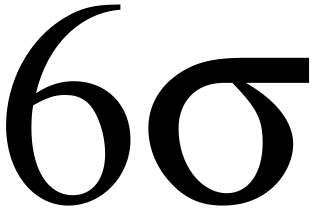
\includegraphics[width=0.35\textwidth]{3-1_normal_distribution/figures/sixsigma}
\end{center}

\ct{\webURL{http://en.wikipedia.org/wiki/Six_Sigma}}

\end{frame}

%%%%%%%%%%%%%%%%%%%%%%%%%%%%%%%%%%%%

\begin{frame}
\frametitle{Quality control}

\dq{{\small At Heinz ketchup factory the amounts which go into bottles of ketchup are supposed to be normally distributed with mean 36 oz. and standard deviation 0.11 oz. Once every 30 minutes a bottle is selected from the production line, and its contents are noted precisely. If the amount of ketchup in the bottle is below 35.8 oz. or above 36.2 oz., then the bottle fails the quality control inspection. What percent of bottles have less than 35.8 ounces of ketchup?}}

\soln{\pause
Let $X$ = amount of ketchup in a bottle: $X \sim N(\mu = 36, \sigma = 0.11)$ \\
\pause
\twocol{0.4}{0.6}{
\begin{center}
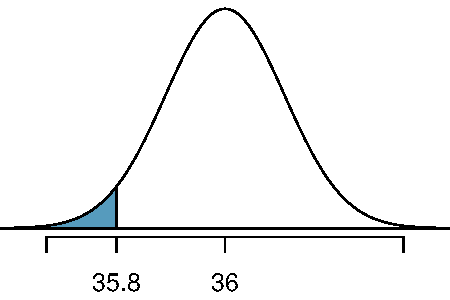
\includegraphics[width=\textwidth]{3-1_normal_distribution/figures/ketchup/ketchupLT358}
\end{center}
}
{
\pause
\[ Z = \frac{35.8 - 36}{0.11} = -1.82 \]
}
}

\end{frame}

%%%%%%%%%%%%%%%%%%%%%%%%%%%%%%%%%%%%

\begin{frame}
\frametitle{Finding the exact probability - using the Z table}

\only<1>{
{\footnotesize
\begin{tabular}{| rrrrr | rrrrr | c}
  \cline{1-10}
&&& \multicolumn{4}{c}{Second decimal place of $Z$} &&& \\
  \cline{1-10}
0.09 &  0.08 &  0.07 &  0.06 &  0.05 &  0.04 &  0.03 &  0.02 &  0.01 &  0.00 & $Z$  \\
    \hline
    \hline
  \tiny{0.0014} & \tiny{0.0014} & \tiny{0.0015} & \tiny{0.0015} & \tiny{0.0016} & \tiny{0.0016} & \tiny{0.0017} & \tiny{0.0018} & \tiny{0.0018} & \tiny{0.0019} & $-2.9$ \\
  \tiny{0.0019} & \tiny{0.0020} & \tiny{0.0021} & \tiny{0.0021} & \tiny{0.0022} & \tiny{0.0023} & \tiny{0.0023} & \tiny{0.0024} & \tiny{0.0025} & \tiny{0.0026} & $-2.8$ \\
  \tiny{0.0026} & \tiny{0.0027} & \tiny{0.0028} & \tiny{0.0029} & \tiny{0.0030} & \tiny{0.0031} & \tiny{0.0032} & \tiny{0.0033} & \tiny{0.0034} & \tiny{0.0035} & $-2.7$ \\
  \tiny{0.0036} & \tiny{0.0037} & \tiny{0.0038} & \tiny{0.0039} & \tiny{0.0040} & \tiny{0.0041} & \tiny{0.0043} & \tiny{0.0044} & \tiny{0.0045} & \tiny{0.0047} & $-2.6$ \\
  \tiny{0.0048} & \tiny{0.0049} & \tiny{0.0051} & \tiny{0.0052} & \tiny{0.0054} & \tiny{0.0055} & \tiny{0.0057} & \tiny{0.0059} & \tiny{0.0060} & \tiny{0.0062} & $-2.5$ \\
    \hline
  \tiny{0.0064} & \tiny{0.0066} & \tiny{0.0068} & \tiny{0.0069} & \tiny{0.0071} & \tiny{0.0073} & \tiny{0.0075} & \tiny{0.0078} & \tiny{0.0080} & \tiny{0.0082} & $-2.4$ \\
  \tiny{0.0084} & \tiny{0.0087} & \tiny{0.0089} & \tiny{0.0091} & \tiny{0.0094} & \tiny{0.0096} & \tiny{0.0099} & \tiny{0.0102} & \tiny{0.0104} & \tiny{0.0107} & $-2.3$ \\
  \tiny{0.0110} & \tiny{0.0113} & \tiny{0.0116} & \tiny{0.0119} & \tiny{0.0122} & \tiny{0.0125} & \tiny{0.0129} & \tiny{0.0132} & \tiny{0.0136} & \tiny{0.0139} & $-2.2$ \\
  \tiny{0.0143} & \tiny{0.0146} & \tiny{0.0150} & \tiny{0.0154} & \tiny{0.0158} & \tiny{0.0162} & \tiny{0.0166} & \tiny{0.0170} & \tiny{0.0174} & \tiny{0.0179} & $-2.1$ \\
  \tiny{0.0183} & \tiny{0.0188} & \tiny{0.0192} & \tiny{0.0197} & \tiny{0.0202} & \tiny{0.0207} & \tiny{0.0212} & \tiny{0.0217} & \tiny{0.0222} & \tiny{0.0228} & $-2.0$ \\
    \hline
  \tiny{0.0233} & \tiny{0.0239} & \tiny{0.0244} & \tiny{0.0250} & \tiny{0.0256} & \tiny{0.0262} & \tiny{0.0268} & \tiny{0.0274} & \tiny{0.0281} & \tiny{0.0287} & $-1.9$ \\
  \tiny{0.0294} & \tiny{0.0301} & \tiny{0.0307} & \tiny{0.0314} & \tiny{0.0322} & \tiny{0.0329} & \tiny{0.0336} & \tiny{0.0344} & \tiny{0.0351} & \tiny{0.0359} & $-1.8$ \\
  \tiny{0.0367} & \tiny{0.0375} & \tiny{0.0384} & \tiny{0.0392} & \tiny{0.0401} & \tiny{0.0409} & \tiny{0.0418} & \tiny{0.0427} & \tiny{0.0436} & \tiny{0.0446} & $-1.7$ \\
  \tiny{0.0455} & \tiny{0.0465} & \tiny{0.0475} & \tiny{0.0485} & \tiny{0.0495} & \tiny{0.0505} & \tiny{0.0516} & \tiny{0.0526} & \tiny{0.0537} & \tiny{0.0548} & $-1.6$ \\
  \tiny{0.0559} & \tiny{0.0571} & \tiny{0.0582} & \tiny{0.0594} & \tiny{0.0606} & \tiny{0.0618} & \tiny{0.0630} & \tiny{0.0643} & \tiny{0.0655} & \tiny{0.0668} & $-1.5$ \\
\hline
\end{tabular}
}}

\soln{
\only<2|handout:0>{
{\footnotesize
\begin{tabular}{| rrrrr | rr>{\columncolor[gray]{0.6}[0pt]}rrr | c}
  \cline{1-10}
&&& \multicolumn{4}{c}{Second decimal place of $Z$} &&& \\
  \cline{1-10}
0.09 &  0.08 &  0.07 &  0.06 &  0.05 &  0.04 &  0.03 &  0.02 &  0.01 &  0.00 & $Z$  \\
    \hline
    \hline
  \tiny{0.0014} & \tiny{0.0014} & \tiny{0.0015} & \tiny{0.0015} & \tiny{0.0016} & \tiny{0.0016} & \tiny{0.0017} & \tiny{0.0018} & \tiny{0.0018} & \tiny{0.0019} & $-2.9$ \\
  \tiny{0.0019} & \tiny{0.0020} & \tiny{0.0021} & \tiny{0.0021} & \tiny{0.0022} & \tiny{0.0023} & \tiny{0.0023} & \tiny{0.0024} & \tiny{0.0025} & \tiny{0.0026} & $-2.8$ \\
  \tiny{0.0026} & \tiny{0.0027} & \tiny{0.0028} & \tiny{0.0029} & \tiny{0.0030} & \tiny{0.0031} & \tiny{0.0032} & \tiny{0.0033} & \tiny{0.0034} & \tiny{0.0035} & $-2.7$ \\
  \tiny{0.0036} & \tiny{0.0037} & \tiny{0.0038} & \tiny{0.0039} & \tiny{0.0040} & \tiny{0.0041} & \tiny{0.0043} & \tiny{0.0044} & \tiny{0.0045} & \tiny{0.0047} & $-2.6$ \\
  \tiny{0.0048} & \tiny{0.0049} & \tiny{0.0051} & \tiny{0.0052} & \tiny{0.0054} & \tiny{0.0055} & \tiny{0.0057} & \tiny{0.0059} & \tiny{0.0060} & \tiny{0.0062} & $-2.5$ \\
    \hline
  \tiny{0.0064} & \tiny{0.0066} & \tiny{0.0068} & \tiny{0.0069} & \tiny{0.0071} & \tiny{0.0073} & \tiny{0.0075} & \tiny{0.0078} & \tiny{0.0080} & \tiny{0.0082} & $-2.4$ \\
  \tiny{0.0084} & \tiny{0.0087} & \tiny{0.0089} & \tiny{0.0091} & \tiny{0.0094} & \tiny{0.0096} & \tiny{0.0099} & \tiny{0.0102} & \tiny{0.0104} & \tiny{0.0107} & $-2.3$ \\
  \tiny{0.0110} & \tiny{0.0113} & \tiny{0.0116} & \tiny{0.0119} & \tiny{0.0122} & \tiny{0.0125} & \tiny{0.0129} & \tiny{0.0132} & \tiny{0.0136} & \tiny{0.0139} & $-2.2$ \\
  \tiny{0.0143} & \tiny{0.0146} & \tiny{0.0150} & \tiny{0.0154} & \tiny{0.0158} & \tiny{0.0162} & \tiny{0.0166} & \tiny{0.0170} & \tiny{0.0174} & \tiny{0.0179} & $-2.1$ \\
  \tiny{0.0183} & \tiny{0.0188} & \tiny{0.0192} & \tiny{0.0197} & \tiny{0.0202} & \tiny{0.0207} & \tiny{0.0212} & \tiny{0.0217} & \tiny{0.0222} & \tiny{0.0228} & $-2.0$ \\
    \hline
  \tiny{0.0233} & \tiny{0.0239} & \tiny{0.0244} & \tiny{0.0250} & \tiny{0.0256} & \tiny{0.0262} & \tiny{0.0268} & \tiny{0.0274} & \tiny{0.0281} & \tiny{0.0287} & $-1.9$ \\
\rowcolor[gray]{.6}
  \tiny{0.0294} & \tiny{0.0301} & \tiny{0.0307} & \tiny{0.0314} & \tiny{0.0322} & \tiny{0.0329} & \tiny{0.0336} & \red{\tiny{0.0344}} & \tiny{0.0351} & \tiny{0.0359} & $-1.8$ \\
  \tiny{0.0367} & \tiny{0.0375} & \tiny{0.0384} & \tiny{0.0392} & \tiny{0.0401} & \tiny{0.0409} & \tiny{0.0418} & \tiny{0.0427} & \tiny{0.0436} & \tiny{0.0446} & $-1.7$ \\
  \tiny{0.0455} & \tiny{0.0465} & \tiny{0.0475} & \tiny{0.0485} & \tiny{0.0495} & \tiny{0.0505} & \tiny{0.0516} & \tiny{0.0526} & \tiny{0.0537} & \tiny{0.0548} & $-1.6$ \\
  \tiny{0.0559} & \tiny{0.0571} & \tiny{0.0582} & \tiny{0.0594} & \tiny{0.0606} & \tiny{0.0618} & \tiny{0.0630} & \tiny{0.0643} & \tiny{0.0655} & \tiny{0.0668} & $-1.5$ \\
\hline
\end{tabular}
}}}

\end{frame}

%%%%%%%%%%%%%%%%%%%%%%%%%%%%%%%%%%%%

%\begin{frame}[fragile]
%\frametitle{Finding the exact probability - using R}
%
%\begin{beamerboxesrounded}[shadow = true, lower = code body]{}
%{\small \begin{verbatim}
%> pnorm(-1.82, mean = 0, sd = 1)
%[1] 0.0344
%\end{verbatim}
%}
%\end{beamerboxesrounded}
%
%$\:$ \\
%\pause
%
%OR
%
%$\:$ \\
%\pause
%
%\begin{beamerboxesrounded}[shadow = true, lower = code body]{}
%{\small \begin{verbatim}
%> pnorm(35.8, mean = 36, sd = 0.11)
%[1] 0.0345
%\end{verbatim}
%}
%\end{beamerboxesrounded}
%
%
%\end{frame}
%
%%%%%%%%%%%%%%%%%%%%%%%%%%%%%%%%%%%%%

\begin{frame}
\frametitle{Practice}

\pq{What percent of bottles \underline{pass} the quality control inspection?}

\vspace{-0.5cm}
\begin{multicols}{2}
\begin{enumerate}[(a)]
\item 1.82\%
\item 3.44\%
\item 6.88\%
\solnMult{93.12\%}
\item 96.56\%
\item[]
\end{enumerate}
\end{multicols}

\soln{
\vspace{-0.5cm}
\pause
\begin{columns}[c]
\column{0.3\textwidth}
\pause
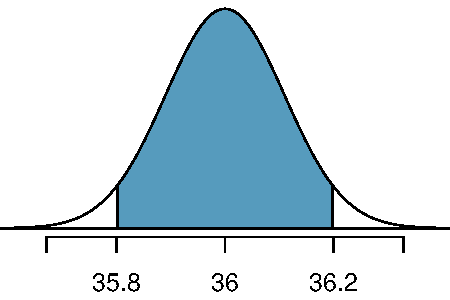
\includegraphics[width=\textwidth]{3-1_normal_distribution/figures/ketchup/ketchupBET}
\column{0.05\textwidth}
=
\pause
\column{0.3\textwidth}
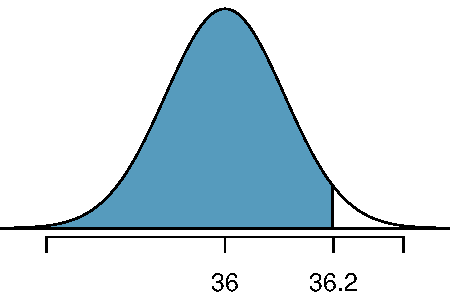
\includegraphics[width=\textwidth]{3-1_normal_distribution/figures/ketchup/ketchupLT362}
\column{0.05\textwidth}
-
\pause
\column{0.3\textwidth}
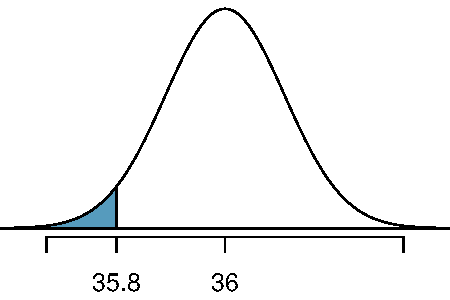
\includegraphics[width=\textwidth]{3-1_normal_distribution/figures/ketchup/ketchupLT358}
\end{columns}
\pause
\begin{eqnarray*}
Z_{35.8} &=& \frac{35.8 - 36}{0.11} = -1.82 \\ \pause
Z_{36.2} &=& \frac{36.2 - 36}{0.11} = 1.82 \\ \pause
P(35.8 < X < 36.2) &=& P(-1.82 < Z < 1.82) = 0.9656 - 0.0344 = 0.9312
\end{eqnarray*}
}

\end{frame}

%%%%%%%%%%%%%%%%%%%%%%%%%%%%%%%%%%%%

\begin{frame}
\frametitle{Finding cutoff points}

\dq{Body temperatures of healthy humans are distributed nearly normally with mean 98.2$\degree$F and standard deviation 0.73$\degree$F. What is the cutoff for the lowest 3\% of human body temperatures?}

\pause

\twocol{0.35}{0.65}
{
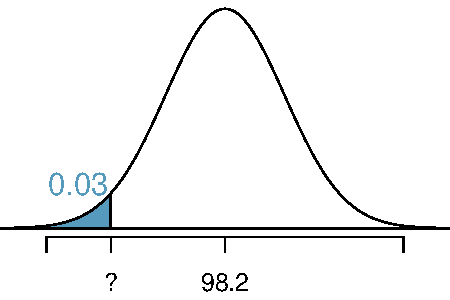
\includegraphics[width=\textwidth]{3-1_normal_distribution/figures/temp/tempLOW3PERC}
}
{
\pause
{\footnotesize
\begin{tabular}{| r >{\columncolor[gray]{0.9}[0pt]}rrrr | c |}
\hline
0.09 &  0.08 &  0.07 &  0.06 &  0.05 & $Z$  \\
    \hline
    \hline
  \tiny{0.0233} & \tiny{0.0239} & \tiny{0.0244} & \tiny{0.0250} & \tiny{0.0256} & $-1.9$ \\
  \rowcolor[gray]{.9}
  \tiny{0.0294} & \tiny{\red{0.0301}} & \tiny{0.0307} & \tiny{0.0314} & \tiny{0.0322} &$-1.8$ \\
  \tiny{0.0367} & \tiny{0.0375} & \tiny{0.0384} & \tiny{0.0392} & \tiny{0.0401} &$-1.7$ \\
\hline
\end{tabular}
}
}
\pause
\begin{eqnarray*}
P(X < x) &=& 0.03 \rightarrow P(Z < \red{-1.88}) = 0.03 \\ \pause
Z &=& \frac{obs~-~mean}{SD} \rightarrow \frac{x - 98.2}{0.73} = -1.88 \\ \pause
x &=& (-1.88 \times 0.73) + 98.2 = 96.8\degree F
\end{eqnarray*}

\ct{Mackowiak, Wasserman, and Levine (1992), \textit{A Critical Appraisal of 98.6 Degrees F, the Upper Limit of the Normal Body Temperature, and Other Legacies of Carl Reinhold August Wunderlick}.}

\end{frame}

%%%%%%%%%%%%%%%%%%%%%%%%%%%%%%%%%%%%

\begin{frame}
\frametitle{Practice}

\pq{Body temperatures of healthy humans are distributed nearly normally with mean 98.2$\degree$F and standard deviation 0.73$\degree$F. What is the cutoff for the highest 10\% of human body temperatures?}

\vspace{-0.5cm}
\begin{multicols}{2}
\begin{enumerate}[(a)]
\item 97.3$\degree$F
\solnMult{99.1$\degree$F}
\item 99.4$\degree$F
\item 99.6$\degree$F
\end{enumerate}
\end{multicols}

\soln{
\vspace{-0.5cm}
\pause
\twocol{0.35}{0.65}
{
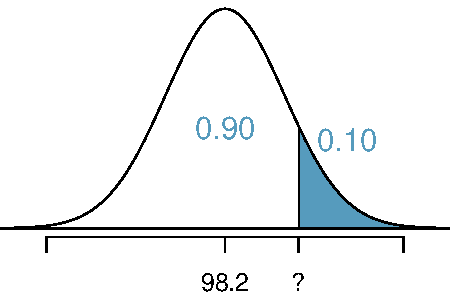
\includegraphics[width=\textwidth]{3-1_normal_distribution/figures/temp/tempHIGH10PERC}
}
{
\pause
{\footnotesize
\begin{tabular}{|c | rrr >{\columncolor[gray]{0.9}[0pt]}rr |}
\hline
$Z$ & 0.05 & 0.06 & 0.07 & 0.08 & 0.09 \\
  \hline
  \hline
  1.0 & \tiny{0.8531} & \tiny{0.8554} & \tiny{0.8577} & \tiny{0.8599} & \tiny{0.8621} \\
  1.1  & \tiny{0.8749} & \tiny{0.8770} & \tiny{0.8790} & \tiny{0.8810} & \tiny{0.8830} \\
   \rowcolor[gray]{.9}
 1.2 & \tiny{0.8944} & \tiny{0.8962} & \tiny{0.8980} & \tiny{\red{0.8997}} & \tiny{0.9015} \\
  1.3 & \tiny{0.9115} & \tiny{0.9131} & \tiny{0.9147} & \tiny{0.9162} & \tiny{0.9177} \\
   \hline
\end{tabular}
}
}
}
\pause
\begin{eqnarray*}
P(X > x) &=& 0.10 \rightarrow P(Z < \red{1.28}) = 0.90 \\ \pause
Z &=& \frac{obs~-~mean}{SD} \rightarrow \frac{x - 98.2}{0.73} = 1.28 \\ \pause
x &=& (1.28 \times 0.73) + 98.2 = 99.1
\end{eqnarray*}

\end{frame}

%%%%%%%%%%%%%%%%%%%%%%%%%%%%%%%%%%%%

\subsection{68-95-99.7 rule}

%%%%%%%%%%%%%%%%%%%%%%%%%%%%%%%%%%%%

\begin{frame}
\frametitle{68-95-99.7 Rule}

\begin{itemize}

\item For nearly normally distributed data, 
\begin{itemize}
\item about 68\% falls within 1 SD of the mean,
\item about 95\% falls within 2 SD of the mean,
\item about 99.7\% falls within 3 SD of the mean.
\end{itemize}

\item It is possible for observations to fall 4, 5, or more standard deviations away from the mean, but these occurrences are very rare if the data are nearly normal.

\end{itemize}

\begin{center}
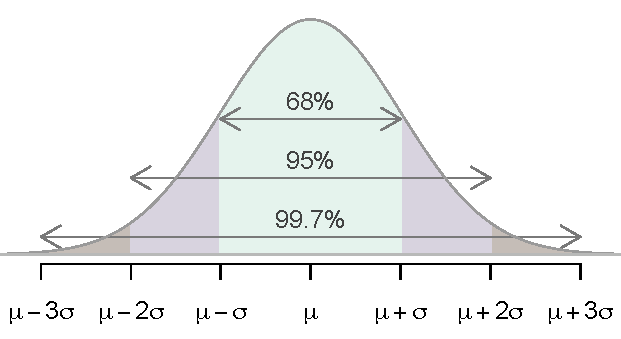
\includegraphics[width=0.7\textwidth]{3-1_normal_distribution/figures/6895997/6895997}
\end{center}

\end{frame}

%%%%%%%%%%%%%%%%%%%%%%%%%%%%%%%%%%%%

\begin{frame}
\frametitle{Describing variability using the 68-95-99.7 Rule}

SAT scores are distributed nearly normally with mean 1500 and standard deviation 300.

\pause
\begin{itemize}

\item $\sim$68\% of students score between 1200 and 1800 on the SAT. 

\item $\sim$95\% of students score between 900 and 2100 on the SAT. 

\item $\sim$99.7\% of students score between 600 and 2400 on the SAT. 

\end{itemize}

\begin{center}
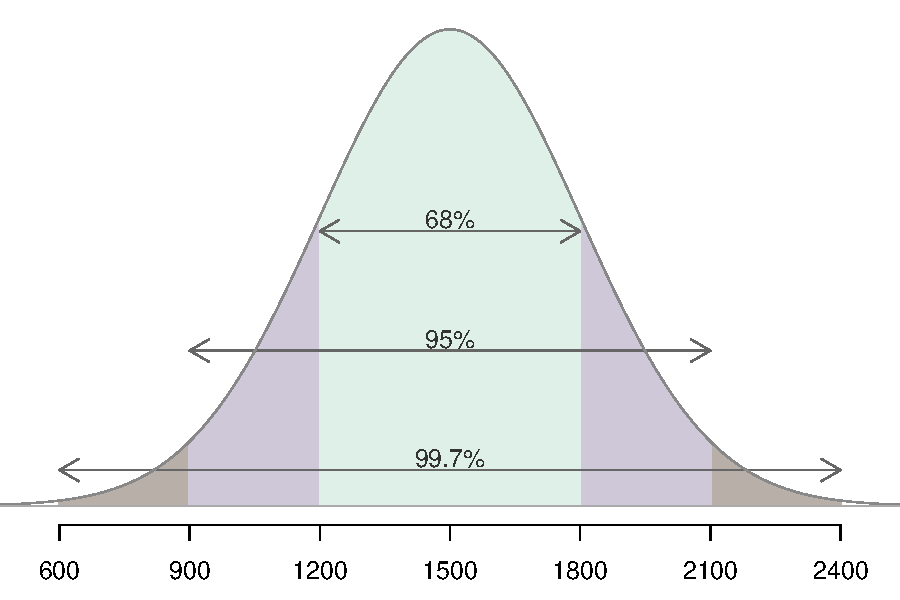
\includegraphics[width=0.65\textwidth]{3-1_normal_distribution/figures/sat_empirical/sat_empirical}
\end{center}

\end{frame}

%%%%%%%%%%%%%%%%%%%%%%%%%%%%%%%%%%%%

\begin{frame}[fragile]
\frametitle{Number of hours of sleep on school nights}

\only<1 | handout:0>{
\begin{center}
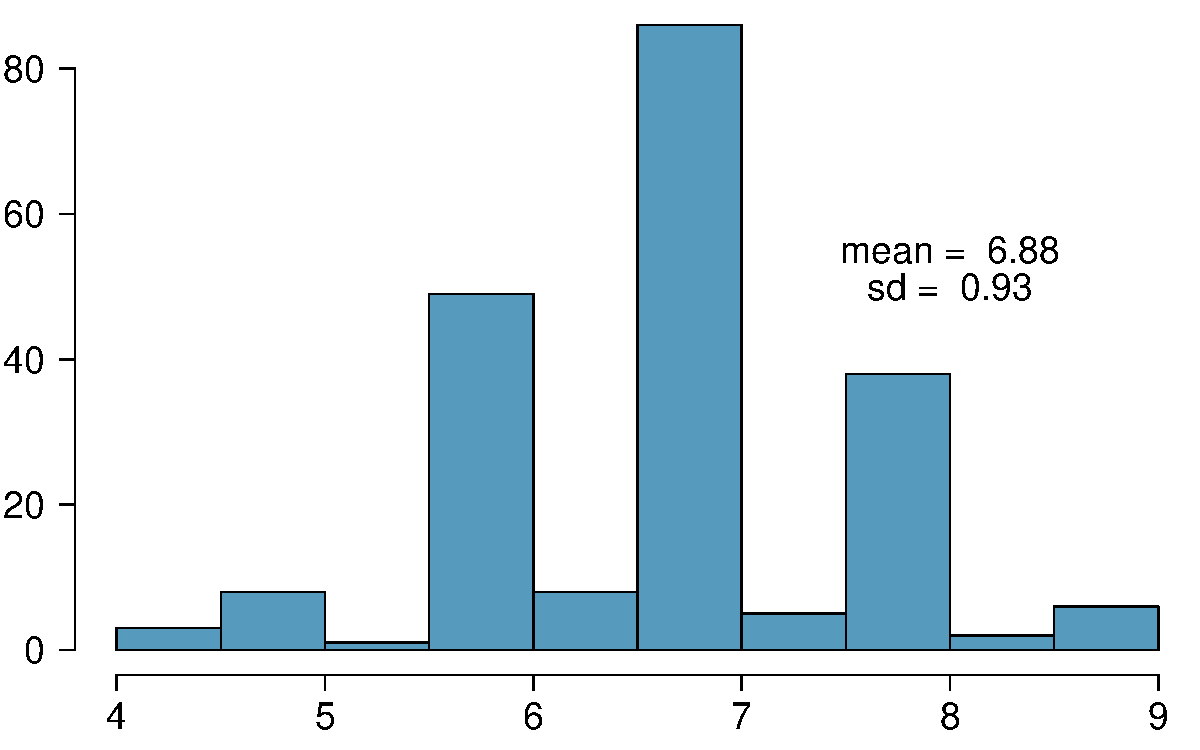
\includegraphics[width=0.75\textwidth]{3-1_normal_distribution/figures/sleep/sleep-hist} 
\end{center}
\vspace{-0.25cm}
\begin{itemize}
\item Mean = 6.88 hours, SD = 0.92 hrs
\item[] \textcolor{white}{72\% of the data are within 1 SD of the mean: $6.88 \pm 0.93$}
\item[] \textcolor{white}{92\% of the data are within 1 SD of the mean: $6.88 \pm 2 \times 0.93$}
\item[] \textcolor{white}{99\% of the data are within 1 SD of the mean: $6.88 \pm 3 \times 0.93$}
\end{itemize}
}

\only<2 | handout:0>{
\begin{center}
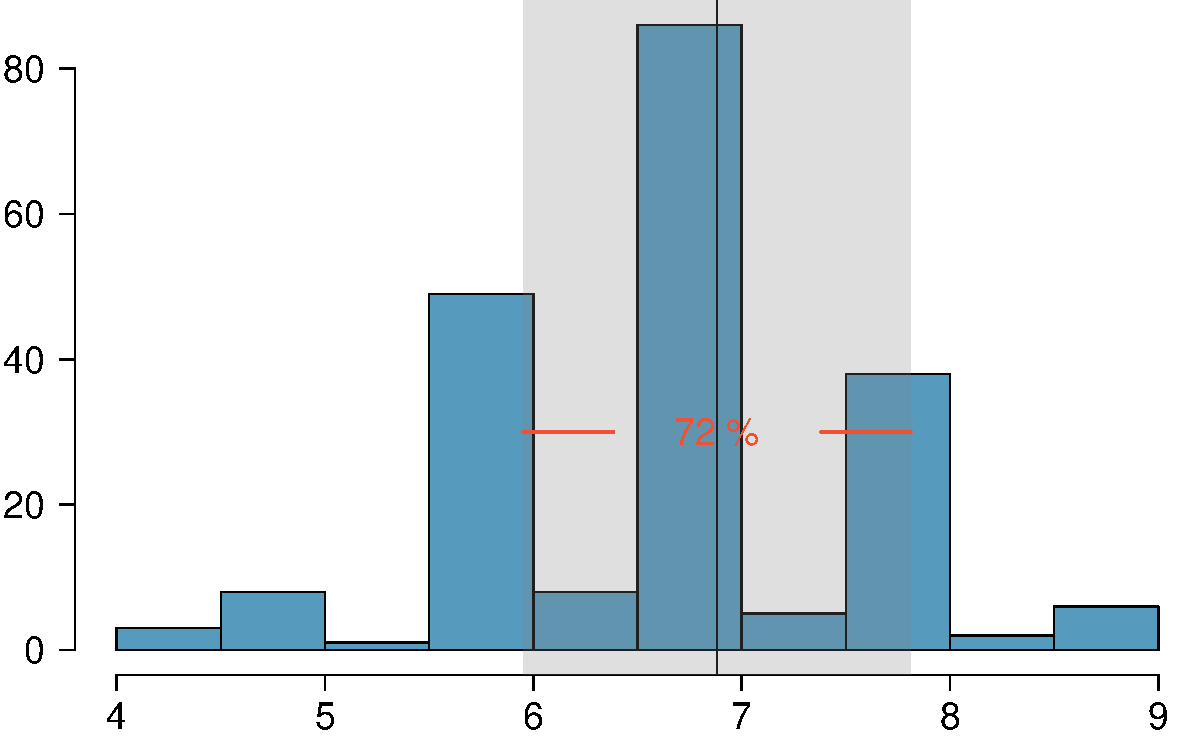
\includegraphics[width=0.75\textwidth]{3-1_normal_distribution/figures/sleep/sleep-hist-sd1} 
\end{center}
\vspace{-0.25cm}
\begin{itemize}
\item Mean = 6.88 hours, SD = 0.92 hrs
\item 72\% of the data are within 1 SD of the mean: $6.88 \pm 0.93$
\item[] \textcolor{white}{92\% of the data are within 1 SD of the mean: $6.88 \pm 2 \times 0.93$}
\item[] \textcolor{white}{99\% of the data are within 1 SD of the mean: $6.88 \pm 3 \times 0.93$}
\end{itemize}
}

\only<3 | handout:0>{
\begin{center}
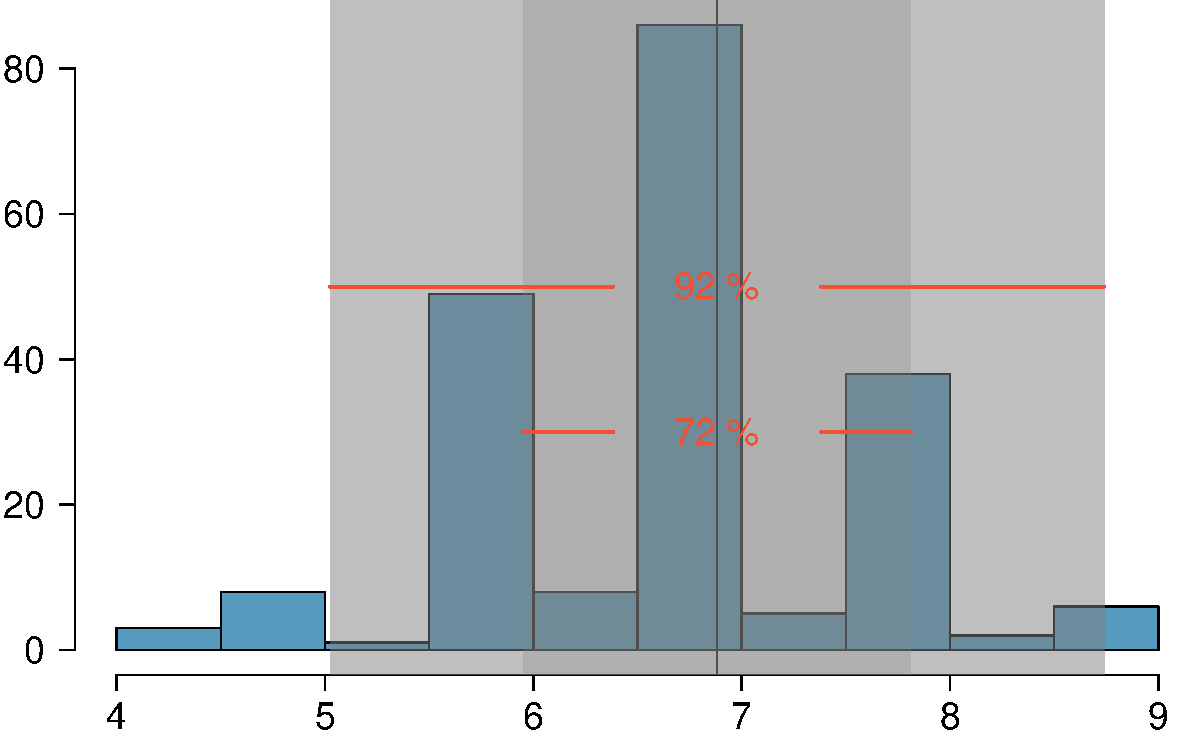
\includegraphics[width=0.75\textwidth]{3-1_normal_distribution/figures/sleep/sleep-hist-sd2} 
\end{center}
\vspace{-0.25cm}
\begin{itemize}
\item Mean = 6.88 hours, SD = 0.92 hrs
\item 72\% of the data are within 1 SD of the mean: $6.88 \pm 0.93$
\item 92\% of the data are within 1 SD of the mean: $6.88 \pm 2 \times 0.93$
\item[] \textcolor{white}{99\% of the data are within 1 SD of the mean: $6.88 \pm 3 \times 0.93$}
\end{itemize}
}

\only<4>{
\begin{center}
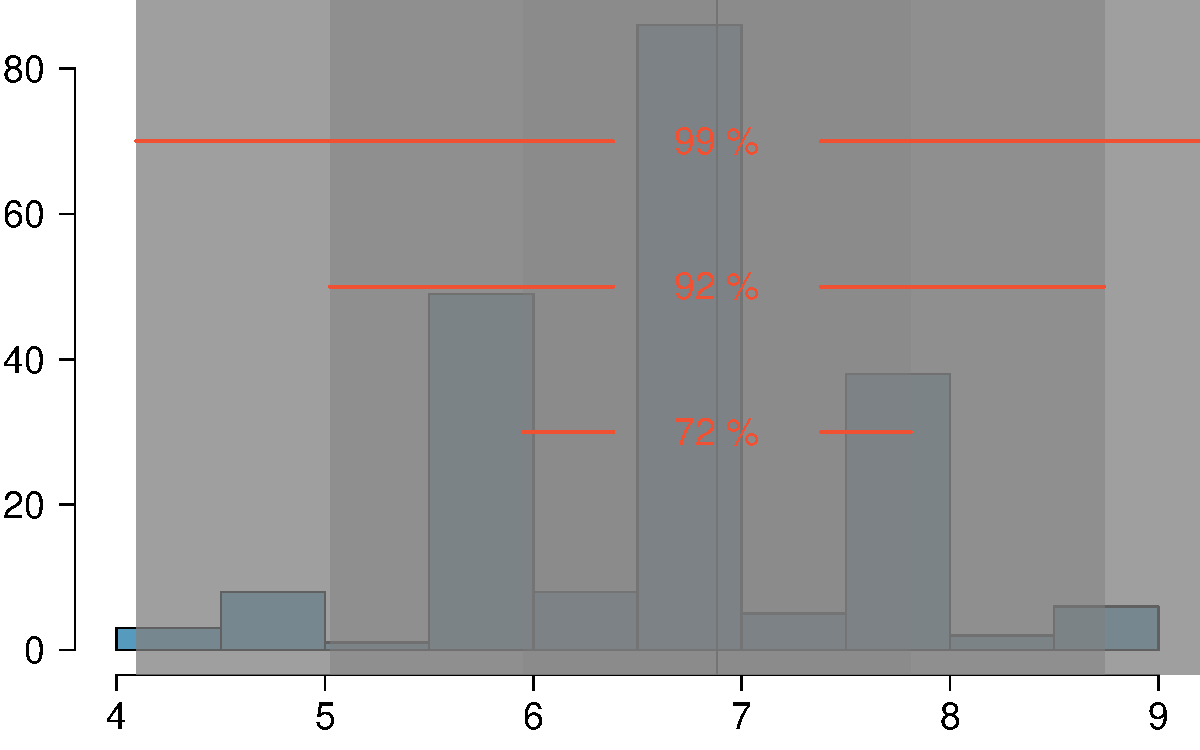
\includegraphics[width=0.75\textwidth]{3-1_normal_distribution/figures/sleep/sleep-hist-sd3} 
\end{center}
\vspace{-0.25cm}
\begin{itemize}
\item Mean = 6.88 hours, SD = 0.92 hrs
\item 72\% of the data are within 1 SD of the mean: $6.88 \pm 0.93$
\item 92\% of the data are within 1 SD of the mean: $6.88 \pm 2 \times 0.93$
\item 99\% of the data are within 1 SD of the mean: $6.88 \pm 3 \times 0.93$
\end{itemize}
}

\end{frame}

%%%%%%%%%%%%%%%%%%%%%%%%%%%%%%%%%%%%

\begin{frame}
\frametitle{Practice}

\pq{Which of the following is \underline{false}?}

\begin{enumerate}[(a)]
\item Majority of Z scores in a right skewed distribution are negative.
\solnMult{In skewed distributions the Z score of the mean might be different than 0.}
\item For a normal distribution, IQR is less than $2 \times SD$.
\item Z scores are helpful for determining how unusual a data point is compared to the rest of the data in the distribution.
\end{enumerate}

\end{frame}

%%%%%%%%%%%%%%%%%%%%%%%%%%%%%%%%%%%%
%%%%%%%%%%%%%%%%%%%%%%%%%%%%%%%%%%%%

\section{Evaluating the normal approximation}

%%%%%%%%%%%%%%%%%%%%%%%%%%%%%%%%%%%%

\subsection{Normal probability plot}

%%%%%%%%%%%%%%%%%%%%%%%%%%%%%%%%%%%%

\begin{frame}
\frametitle{Normal probability plot}

A histogram and \hl{normal probability plot} of a sample of 100 male heights.

\begin{center}
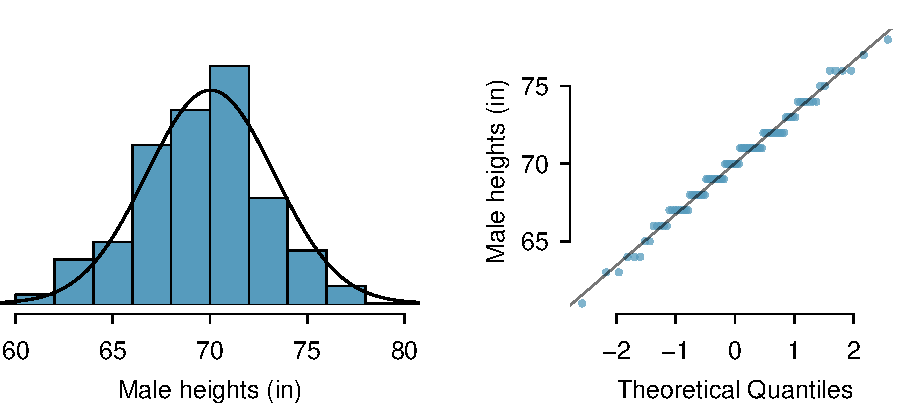
\includegraphics[width=0.9\textwidth]{3-2_evaluating_normal_approx/figures/fcidMHeights/fcidMHeights}
\end{center}

\end{frame}

%%%%%%%%%%%%%%%%%%%%%%%%%%%%%%%%%%%%

\begin{frame}
\frametitle{Anatomy of a normal probability plot}

\begin{itemize}

\item Data are plotted on the y-axis of a normal probability plot, and theoretical quantiles (following a normal distribution) on the x-axis.

\item If there is a linear relationship in the plot, then the data follow a nearly normal distribution.

\item Constructing a normal probability plot requires calculating percentiles and corresponding z-scores for each observation, which is tedious. Therefore we generally rely on software when making these plots.

\end{itemize}

\end{frame}

%%%%%%%%%%%%%%%%%%%%%%%%%%%%%%%%%%%%

\begin{frame}

\dq{Below is a histogram and normal probability plot for the NBA heights from the 2008-2009 season. Do these data appear to follow a normal distribution?}

\begin{center}
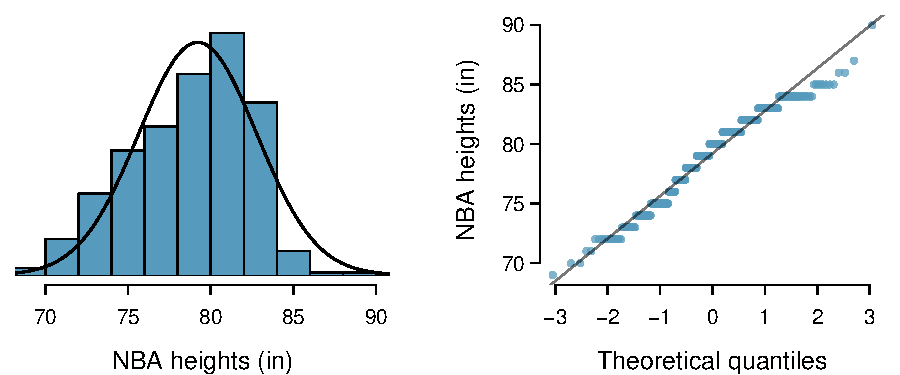
\includegraphics[width=0.8\textwidth]{3-2_evaluating_normal_approx/figures/nbaNormal/nbaNormal}
\end{center}

\pause

\dq{Why do the points on the normal probability have jumps?}

\end{frame}

%%%%%%%%%%%%%%%%%%%%%%%%%%%%%%%%%%%%

\begin{frame}
\frametitle{Normal probability plot and skewness}

\twocol{0.2}{0.8}{
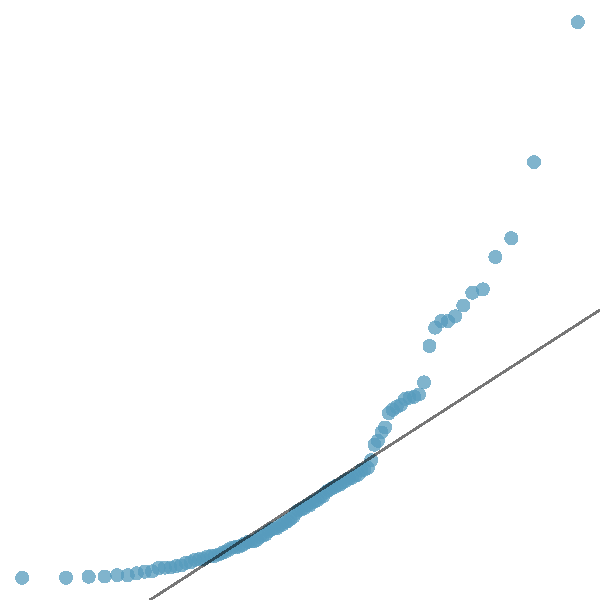
\includegraphics[width=0.8\textwidth]{3-2_evaluating_normal_approx/figures/skew/qq_rs}
}
{
Right skew - Points bend up and to the left of the line.
}

\twocol{0.2}{0.8}{
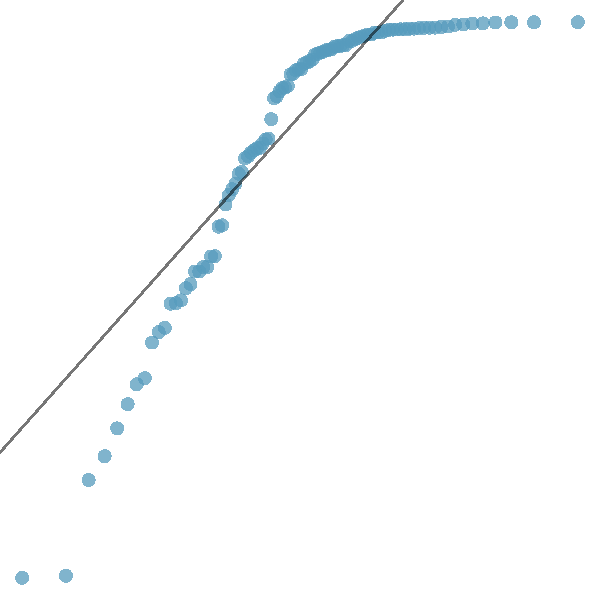
\includegraphics[width=0.8\textwidth]{3-2_evaluating_normal_approx/figures/skew/qq_ls}
}
{
Left skew- Points bend down and to the right of the line.
}

\twocol{0.2}{0.8}{
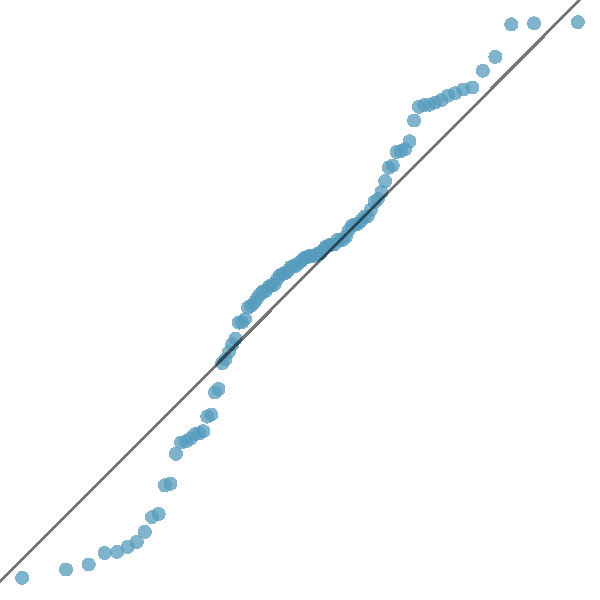
\includegraphics[width=0.8\textwidth]{3-2_evaluating_normal_approx/figures/skew/qq_st}
}
{
Short tails (narrower than the normal distribution) - Points follow an S shaped-curve.
}

\twocol{0.2}{0.8}{
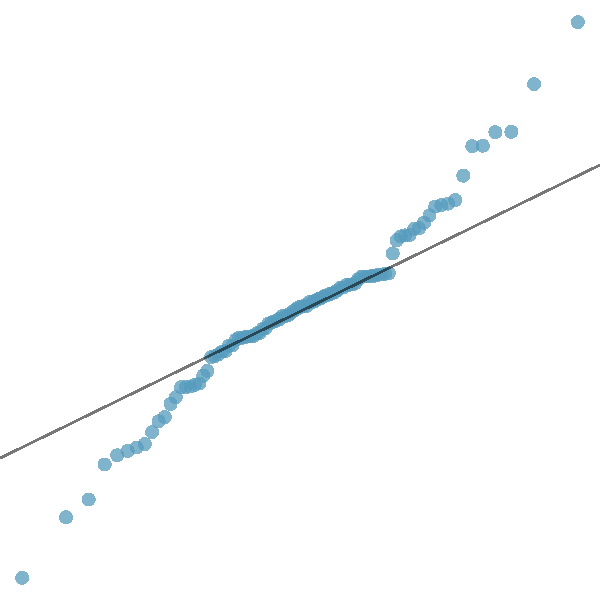
\includegraphics[width=0.8\textwidth]{3-2_evaluating_normal_approx/figures/skew/qq_lt}
}
{
Long tails (wider than the normal distribution) - Points start below the line, bend to follow it, and end above it.
}

\end{frame}

%%%%%%%%%%%%%%%%%%%%%%%%%%%%%%%%%%%%
%%%%%%%%%%%%%%%%%%%%%%%%%%%%%%%%%%%%

\section{Geometric distribution}

%%%%%%%%%%%%%%%%%%%%%%%%%%%%%%%%%%%%

\subsection{Bernoulli distribution}

\begin{frame}
\frametitle{Milgram experiment}

\twocol{0.6}{0.4}{

\begin{itemize}

\item Stanley Milgram, a Yale University psychologist, conducted a series of experiments on obedience to authority starting in 1963. 

\item Experimenter (E) orders the teacher (T), the subject of the experiment, to give severe electric shocks to a learner (L) each time the learner answers a question incorrectly. 

\item The learner is actually an actor, and the electric shocks are not real, but a prerecorded sound is played each time the teacher administers an electric shock.

\end{itemize}

}
{
\begin{center}
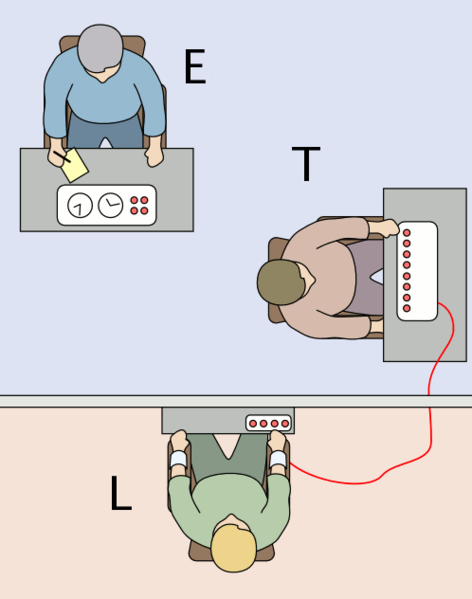
\includegraphics[width=\textwidth]{3-3_geometric_distribution/figures/milgram}
\end{center}
\ct{\webURL{http://en.wikipedia.org/wiki/File:Milgram_Experiment_v2.png}}
}

\end{frame}

%%%%%%%%%%%%%%%%%%%%%%%%%%%%%%%%%%%%

\begin{frame}
\frametitle{Milgram experiment (cont.)}

\begin{itemize}

\item These experiments measured the willingness of study participants to obey an authority figure who instructed them to perform acts that conflicted with their personal conscience.

\item Milgram found that about 65\% of people would obey authority and give such shocks.

\item Over the years, additional research suggested this number is approximately consistent across communities and time.

\end{itemize}

\end{frame}


%%%%%%%%%%%%%%%%%%%%%%%%%%%%%%%%%%%%

\begin{frame}
\frametitle{Bernouilli random variables}

\begin{itemize}

\item Each person in Milgram's experiment can be thought of as a \hl{trial}.

\item A person is labeled a \hl{success} if she refuses to administer a severe shock, and \hl{failure} if she administers such shock.

\item Since only 35\% of people refused to administer a shock, \hl{probability of success} is \mathhl{p = 0.35}.

\item When an individual trial has only two possible outcomes, it is called a \hl{Bernoulli random variable}.

\end{itemize}

\end{frame}

%%%%%%%%%%%%%%%%%%%%%%%%%%%%%%%%%%%%

\subsection{Geometric distribution}

\begin{frame}
\frametitle{Geometric distribution}

{\small

\dq{Dr. Smith wants to repeat Milgram's experiments but she only wants to sample people until she finds someone who will not inflict a severe shock. What is the probability that she stops after the first person?}

\[ P(1^{st}~person~refuses) = 0.35 \]

\pause

\dq{... the third person?}
\[ P(1^{st}~and~2^{nd}~shock,~3^{rd}~refuses) = \slot{S}{0.65} \times \slot{S}{0.65} \times  \slot{R}{0.35} = 0.65^2 \times 0.35 \approx 0.15 \]

\pause

\dq{... the tenth person?}
\soln{
\pause
\[ P(9~shock,~10^{th}~refuses) = \underbrace{\slot{S}{0.65} \times \cdots \times \slot{S}{0.65}}_{9~of~these} \times  \slot{R}{0.35} = 0.65^9 \times 0.35 \approx 0.0072 \]
}
}

\end{frame}

%%%%%%%%%%%%%%%%%%%%%%%%%%%%%%%%%%%%

\begin{frame}
\frametitle{Geometric distribution (cont.)}

\hl{Geometric distribution} describes the waiting time until a success for \hl{independent and identically distributed (iid)} Bernouilli random variables.
\begin{itemize}
\item independence: outcomes of trials don't affect each other
\item identical: the probability of success is the same for each trial
\end{itemize}

$\:$ \\
$\:$ \\

\pause

\formula{Geometric probabilities}{If $p$ represents probability of success, $(1-p)$ represents probability of failure, and $n$ represents number of independent trials \[P(success~on~the~n^{th}~trial) = (1-p)^{n-1} p\]}

\end{frame}

%%%%%%%%%%%%%%%%%%%%%%%%%%%%%%%%%%%%

\begin{frame}

\pq{Can we calculate the probability of rolling a 6 for the first time on the 6$^{th}$ roll of a die using the geometric distribution? Note that what was a success (rolling a 6) and what was a failure (not rolling a 6) are clearly defined and one or the other must happen for each trial.}

\begin{enumerate}[(a)]
\item no, on the roll of a die there are more than 2 possible outcomes
\only<1>{\item yes, why not}
\soln{\only<2>{\item \orange{yes, why not}}}
\end{enumerate}

\soln{
\only<2>{
\[P(6~on~the~6^{th}~roll) = \pr{ \frac{5}{6} }^5 \pr{ \frac{1}{6} } \approx 0.067 \]
}
}

\end{frame}

%%%%%%%%%%%%%%%%%%%%%%%%%%%%%%%%%%%%

\begin{frame}
\frametitle{Expected value}

\dq{How many people is Dr. Smith expected to test before finding the first one that refuses to administer the shock?}

\pause

The expected value, or the mean, of a geometric distribution is defined as $\frac{1}{p}$.
\[ \mu = \frac{1}{p} = \frac{1}{0.35} = 2.86 \]

\pause

She is expected to test 2.86 people before finding the first one that refuses to administer the shock. 

\pause

But how can she test a non-whole number of people?

\end{frame}

%%%%%%%%%%%%%%%%%%%%%%%%%%%%%%%%%%%%

\begin{frame}
\frametitle{Expected value and its variability}

\formula{Mean and standard deviation of geometric distribution}{
\[ \mu = \frac{1}{p} \qquad \qquad \sigma = \sqrt{\frac{1-p}{p^2}} \] 
}

\pause

\begin{itemize}

\item Going back to Dr. Smith's experiment:

\[ \sigma = \sqrt{\frac{1-p}{p^2}} = \sqrt{\frac{1-0.35}{0.35^2}} = 2.3 \]

\pause

\item Dr. Smith is expected to test 2.86 people before finding the first one that refuses to administer the shock, give or take 2.3 people.

\pause

\item These values only make sense in the context of repeating the experiment many many times.

\end{itemize}

\end{frame}

%%%%%%%%%%%%%%%%%%%%%%%%%%%%%%%%%%%%
%%%%%%%%%%%%%%%%%%%%%%%%%%%%%%%%%%%%

\section{Binomial distribution}

%%%%%%%%%%%%%%%%%%%%%%%%%%%%%%%%%%%%

\subsection{The binomial distribution}

%%%%%%%%%%%%%%%%%%%%%%%%%%%%%%%%%%%%

\begin{frame}

\dq{Suppose we randomly select four individuals to participate in this experiment. What is the probability that exactly 1 of them will refuse to administer the shock?}
\pause
Let's call these people Allen (A), Brittany (B), Caroline (C), and Damian (D). Each one of the four scenarios below will satisfy the condition of ``exactly 1 of them refuses to administer the shock": \\
\vspace{0.25cm}
\pause
\begin{changemargin}{+1.5cm}{+0cm}
{\footnotesize
\begin{enumerate}
\item[Scenario 1:] $\slot{0.35}{\text{(A) \red{refuse}}} \times \slot{0.65}{\text{(B) shock}} \times \slot{0.65}{\text{(C) shock}} \times \slot{0.65}{\text{(D) shock}} = 0.0961$
\pause
\item[Scenario 2:] $\slot{0.65}{\text{(A) shock}} \times \slot{0.35}{\text{(B) \red{refuse}}}\times \slot{0.65}{\text{(C) shock}} \times \slot{0.65}{\text{(D) shock}} = 0.0961$
\pause
\item[Scenario 3:] $\slot{0.65}{\text{(A) shock}} \times \slot{0.65}{\text{(B) shock}} \times \slot{0.35}{\text{(C) \red{refuse}}}\times \slot{0.65}{\text{(D) shock}} = 0.0961$
\pause
\item[Scenario 4:] $\slot{0.65}{\text{(A) shock}} \times \slot{0.65}{\text{(B) shock}} \times \slot{0.65}{\text{(C) shock}} \times \slot{0.35}{\text{(D) \red{refuse}}} = 0.0961$
\end{enumerate}
}
\end{changemargin}
\pause
The probability of exactly one 1 of 4 people refusing to administer the shock is the sum of all of these probabilities.
\[ 0.0961+ 0.0961 + 0.0961 + 0.0961 = 4 \times 0.0961 = 0.3844 \]

\end{frame}

%%%%%%%%%%%%%%%%%%%%%%%%%%%%%%%%%%%%

\begin{frame}
\frametitle{Binomial distribution}

The question from the prior slide asked for the probability of given number of successes, \mathhl{k}, in a given number of trials, \mathhl{n}, ($k = 1$ success in $n = 4$ trials), and we calculated this probability as
\[ \#~of~scenarios \times P(single~scenario) \]

\pause

\begin{itemize}

\item $\#~of~scenarios$: there is a less tedious way to figure this out, we'll get to that shortly...

\pause

\item $P(single~scenario) = p^k~(1-p)^{(n-k)}$ \\
{\tiny probability of success to the power of number of successes, probability of failure to the power of number of failures}

\end{itemize}

\pause

The \hl{Binomial distribution} describes the probability of having exactly $k$ successes in $n$ independent Bernouilli trials with probability of success $p$.

\end{frame}

%%%%%%%%%%%%%%%%%%%%%%%%%%%%%%%%%%%%

\begin{frame}
\frametitle{Counting the \# of scenarios}

Earlier we wrote out all possible scenarios that fit the condition of exactly one person refusing to administer the shock. If $n$ was larger and/or $k$ was different than 1, for example, $n = 9$ and $k = 2$:

\pause

\begin{center}
\begin{tabular}{c}
\red{R}\red{R}SSSSSSS \\ 
\pause
S\red{R}\red{R}SSSSSS \\
\pause
SS\red{R}\red{R}SSSSS \\
$\cdots$ \\
SS\red{R}SS\red{R}SSS \\
$\cdots$ \\
SSSSSSS\red{R}\red{R} \\
\end{tabular}
\end{center}

writing out all possible scenarios would be incredibly tedious and prone to errors.

\end{frame}

%%%%%%%%%%%%%%%%%%%%%%%%%%%%%%%%%%%%

\begin{frame}[fragile]
\frametitle{Calculating the \# of scenarios}

\formula{Choose function}
{
The \hl{choose function} is useful for calculating the number of ways to choose $k$ successes in $n$ trials.
\[ {n \choose k} = \frac{n!}{k! (n - k)!} \]
}

\pause

\begin{itemize}

\item $k = 1$, $n = 4$: ${4 \choose 1} = \frac{4!}{1! (4 - 1)!} = \frac{4 \times 3 \times 2 \times 1}{1 \times (3 \times 2 \times 1)} = 4$

\pause

\item $k = 2$, $n = 9$: ${9 \choose 2} = \frac{9!}{2! (9 - 1)!} = \frac{9 \times 8 \times 7!}{2 \times 1 \times 7!} = \frac{72}{2} = 36$

\end{itemize}

\vfill

\Note{You can also use R for these calculations:}
\begin{beamerboxesrounded}[shadow = true, lower = code body]{}
{\small
\begin{verbatim}
> choose(9,2)
[1] 36
\end{verbatim}
}
\end{beamerboxesrounded}

\end{frame}

%%%%%%%%%%%%%%%%%%%%%%%%%%%%%%%%%%%

\begin{frame}[fragile]
\frametitle{Properties of the choose function}

\pq{Which of the following is false?}

\begin{enumerate}[(a)]
\item There are $n$ ways of getting 1 success in $n$ trials, ${n \choose 1} = n$.
\item There is only 1 way of getting $n$ successes in $n$ trials, ${n \choose n} = 1$.
\item There is only 1 way of getting $n$ failures in $n$ trials, ${n \choose 0} = 1$.
\solnMult{There are $n-1$ ways of getting $n-1$ successes in $n$ trials, ${n \choose n-1} = n-1$.}
\end{enumerate}

\end{frame}

%%%%%%%%%%%%%%%%%%%%%%%%%%%%%%%%%%%

\begin{frame}
\frametitle{Binomial distribution (cont.)}

\formula{Binomial probabilities}
{
If $p$ represents probability of success, $(1-p)$ represents probability of failure, $n$ represents number of independent trials, and $k$ represents number of successes 
\[P(k~successes~in~n~trials) = {n \choose k}~p^k~(1-p)^{(n-k)} \]
} 


\end{frame}

%%%%%%%%%%%%%%%%%%%%%%%%%%%%%%%%%%%

\begin{frame}

\pq{Which of the following is not a condition that needs to be met for the binomial distribution to be applicable?}

\begin{enumerate}[(a)]
\item the trials must be independent
\item the number of trials, $n$, must be fixed
\item each trial outcome must be classified as a \textit{success} or a \textit{failure}
\solnMult{the number of desired successes, $k$, must be greater than the number of trials}
\item the probability of success, $p$, must be the same for each trial
\end{enumerate}

\end{frame}

%%%%%%%%%%%%%%%%%%%%%%%%%%%%%%%%%%%

\begin{frame}
\frametitle{}

\pq{A 2012 Gallup survey suggests that 26.2\% of Americans are obese. Among a random sample of 10 Americans, what is the probability that exactly 8 are obese?}

\begin{enumerate}[(a)]
\item pretty high
\solnMult{pretty low}
\end{enumerate}

\vfill

\ct{Gallup: \webURL{http://www.gallup.com/poll/160061/obesity-rate-stable-2012.aspx}, January 23, 2013.} 

\end{frame}

%%%%%%%%%%%%%%%%%%%%%%%%%%%%%%%%%%%%

\begin{frame}

\pq{A 2012 Gallup survey suggests that 26.2\% of Americans are obese. Among a random sample of 10 Americans, what is the probability that exactly 8 are obese?}

\begin{enumerate}[(a)]
\item $0.262^8 \times 0.738^2$
\item ${8 \choose 10} \times 0.262^8 \times 0.738^2$
\solnMult{${10 \choose 8} \times 0.262^8 \times 0.738^2$} \soln{\red{\only<2>{$ = 45 \times  0.262^8 \times 0.738^2 = 0.0005$}}}
\item ${10 \choose 8} \times 0.262^2 \times 0.738^8$
\end{enumerate}



\end{frame}

%%%%%%%%%%%%%%%%%%%%%%%%%%%%%%%%%%%

\begin{frame}
\frametitle{The birthday problem}

\dq{What is the probability that 2 randomly chosen people share a birthday?}

\pause

Pretty low, $\frac{1}{365} \approx 0.0027$.

\pause

\dq{What is the probability that at least 2 people out of 366 people share a birthday?}

\pause

Exactly 1! (Excluding the possibility of a leap year birthday.)

\end{frame}

%%%%%%%%%%%%%%%%%%%%%%%%%%%%%%%%%%%

\begin{frame}
\frametitle{The birthday problem (cont.)}

\dq{What is the probability that at least 2 people (1 match) out of 121 people share a birthday?}

\pause

Somewhat complicated to calculate, but we can think of it as the complement of the probability that there are no matches in 121 people.

\vspace{-0.75cm}

\begin{eqnarray*}
P(no~matches) &=& 1 \times \pr{1 - \frac{1}{365}} \times \pr{1 - \frac{2}{365}} \times \cdots \times \pr{1 - \frac{120}{365}} \\
\pause
&=& \frac{365 \times 364 \times \cdots \times 245}{365^{121}} \\
\pause
&=& \frac{365!}{365^{121} \times (365-121)!} \\
\pause
&=& \frac{121! \times {365 \choose 121}}{365^{121}} 
\pause
\approx 0 \\
\pause
P(at~least~1~match) &\approx& 1
\end{eqnarray*}

\end{frame}


%%%%%%%%%%%%%%%%%%%%%%%%%%%%%%%%%%%

\begin{frame}
\frametitle{Expected value}

\dq{A 2012 Gallup survey suggests that 26.2\% of Americans are obese. \\  

Among a random sample of 100 Americans, how many would you expect to be obese?}

\pause

\begin{itemize}

\item Easy enough, $100 \times 0.262 = 26.2$.

\pause

\item Or more formally, $\mu = np = 100 \times 0.262 = 26.2$.

\pause

\item But this doesn't mean in every random sample of 100 people exactly 26.2 will be obese. In fact, that's not even possible. In some samples this value will be less, and in others more. How much would we expect this value to vary?

\end{itemize}

\end{frame}

%%%%%%%%%%%%%%%%%%%%%%%%%%%%%%%%%%%

\begin{frame}
\frametitle{Expected value and its variability}

\formula{Mean and standard deviation of binomial distribution}
{\[ \mu = np \qquad \qquad \sigma = \sqrt{np(1-p)} \] }

\pause

\begin{itemize}

\item Going back to the obesity rate:

\[ \sigma = \sqrt{np(1-p)} = \sqrt{100 \times 0.262 \times 0.738} \approx  4.4\]

\pause

\item We would expect 26.2 out of 100 randomly sampled Americans to be obese, with a standard deviation of 4.4.

\end{itemize}

\Note{Mean and standard deviation of a binomial might not always be whole numbers, and that is alright, these values represent what we would expect to see on average.}

\end{frame}

%%%%%%%%%%%%%%%%%%%%%%%%%%%%%%%%%%%

\begin{frame}
\frametitle{Unusual observations}

Using the notion that \hl{observations that are more than 2 standard deviations away from the mean are considered unusual} and the mean and the standard deviation we just computed, we can calculate a range for the plausible number of obese Americans in random samples of 100.

\[ 26.2 \pm (2 \times 4.4) = (17.4, 35) \]

\end{frame}

%%%%%%%%%%%%%%%%%%%%%%%%%%%%%%%%%%%

\begin{frame}

\pq{An August 2012 Gallup poll suggests that 13\% of Americans think home schooling provides an excellent education for children.  Would a random sample of 1,000 Americans where only 100 share this opinion be considered unusual?}
\begin{multicols}{2}
\begin{enumerate}[(a)]
\item No
\solnMult{Yes}
\end{enumerate}
\end{multicols}

\only<1>{
\begin{center}
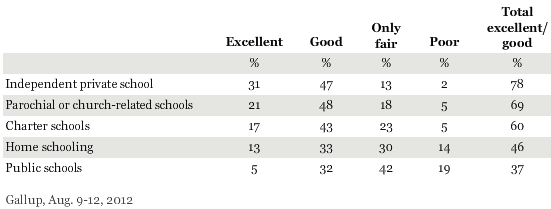
\includegraphics[width=0.8\textwidth]{3-4_binomial_distribution/figures/homeschool}
\end{center}
}

\vspace{-0.5cm}
\soln{
{\small
\only<2->{
\begin{align*}
\mu &= np = 1,000 \times 0.13 = 130 \\
\sigma &= \sqrt{np(1-p)} = \sqrt{1,000 \times 0.13 \times 0.87} \approx 10.6
\end{align*}
}
\begin{changemargin}{+1cm}{+0cm}
\pause
\begin{enumerate}
\only<3->{\item[Method 1:] Range of usual observations: $130 \pm 2 \times 10.6 = (108.8, 151.2)$ \\
100 is outside this range, so would be considered unusual.}
\only<4->{\item[Method 2:] Z-score of observation: $Z = \frac{x - mean}{SD} = \frac{100 - 130}{10.6} = -2.83$ \\
100 is more than 2 SD below the mean, so would be considered unusual.}
\end{enumerate}
\end{changemargin}
}}

\vfill

\ct{\webURL{http://www.gallup.com/poll/156974/private-schools-top-marks-educating-children.aspx}}

\end{frame}

%%%%%%%%%%%%%%%%%%%%%%%%%%%%%%%%%%%%

\subsection{Normal approximation to the binomial}

%%%%%%%%%%%%%%%%%%%%%%%%%%%%%%%%%%%%

\begin{frame}
\frametitle{}

\app{Shapes of binomial distributions}
{
For this activity you will use a web applet. Go to \webURL{http://socr.stat.ucla.edu/htmls/SOCR_Experiments.html} and choose Binomial coin experiment in the drop down menu on the left.
\begin{itemize}
\item Set the number of trials to 20 and the probability of success to 0.15. Describe the shape of the distribution of number of successes. 
\item Keeping $p$ constant at 0.15, determine the minimum sample size required to obtain a unimodal and symmetric distribution of number of successes. Please submit only one response per team.
\item Further considerations:
\begin{itemize}
\item What happens to the shape of the distribution as $n$ stays constant and $p$ changes?
\item What happens to the shape of the distribution as $p$ stays constant and $n$ changes?
\end{itemize}
\end{itemize}
}

\end{frame}

%%%%%%%%%%%%%%%%%%%%%%%%%%%%%%%%%%%%

\begin{frame}
\frametitle{Distributions of number of successes}

\dq{Hollow histograms of samples from the binomial model where $p = 0.10$ and $n = 10$, $30$, $100$, and $300$. What happens as $n$ increases?}

\begin{center}
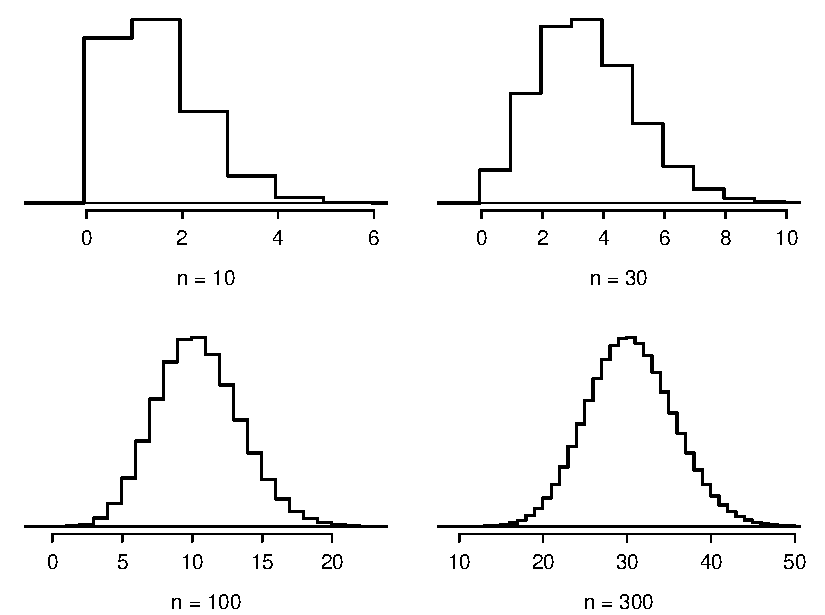
\includegraphics[width=0.60\textwidth]{3-4_binomial_distribution/figures/fourBinomialModelsShowingApproxToNormal/fourBinomialModelsShowingApproxToNormal}
\end{center}

\end{frame}

%%%%%%%%%%%%%%%%%%%%%%%%%%%%%%%%%%%

\begin{frame}
\frametitle{Low large is large enough?}

The sample size is considered large enough if the expected number of successes and failures are both at least 10.
\[ np \ge 10 \qquad \text{ and } \qquad n(1-p) \ge 10 \]

\soln{\only<2->{$10 \times 0.13 = 1.3; 10 \times (1 - 0.13) = 8.7$}}

\end{frame}

%%%%%%%%%%%%%%%%%%%%%%%%%%%%%%%%%%

\begin{frame}
\frametitle{}

\pq{Below are four pairs of Binomial distribution parameters. Which distribution can be approximated by the normal distribution?}

\begin{enumerate}[(a)]
\item $n = 100, p = 0.95$
\solnMult{$n = 25, p = 0.45$} \soln{\only<2>{\red{$\rightarrow 25 \times 0.45 = 11.25; 25 \times 0.55 = 13.75$}}}
\item $n = 150, p = 0.05$
\item $n = 500, p = 0.015$
\end{enumerate}

\end{frame}


%%%%%%%%%%%%%%%%%%%%%%%%%%%%%%%%%%%%

\begin{frame}
\frametitle{An analysis of Facebook users}

\dq{A recent study found that ``Facebook users get more than they give". For example:
\begin{itemize}
\item 40\% of Facebook users in our sample made a friend request, but 63\% received at least one request
\item Users in our sample pressed the like button next to friends' content an average of 14 times, but had their content ``liked" an average of 20 times
\item Users sent 9 personal messages, but received 12
\item 12\% of users tagged a friend in a photo, but 35\% were themselves tagged in a photo
\end{itemize}
Any guesses for how this pattern can be explained?
}

\soln{\only<2>{Power users contribute much more content than the typical user.}}

\ct{\webURL{http://www.pewinternet.org/Reports/2012/Facebook-users/Summary.aspx}}

\end{frame}

%%%%%%%%%%%%%%%%%%%%%%%%%%%%%%%%%%%

\begin{frame}
\frametitle{}

\dq{This study also found that approximately 25\% of Facebook users are considered power users. The same study found that the average Facebook user has 245 friends. What is the probability that the average Facebook user with 245 friends has 70 or more friends who would be considered power users? Note any assumptions you must make.}

We are given that $n = 245, p = 0.25$, and we are asked for the probability $P(K \ge 70)$. To proceed, we need independence, which we'll assume but could check if we had access to more Facebook data.

\pause

\begin{align*}
P(X \ge 70) &= P(K = 70\text{ or }K = 71\text{ or }K = 72\text{ or }\cdots\text{ or } K = 245) \\
&= P(K = 70) + P(K = 71) + P(K = 72) + \cdots + P(K = 245)
\end{align*}

\pause

This seems like an awful lot of work...

\end{frame}

%%%%%%%%%%%%%%%%%%%%%%%%%%%%%%%%%%%%

\begin{frame}
\frametitle{Normal approximation to the binomial}

When the sample size is large enough, the binomial distribution with parameters $n$ and $p$ can be approximated by the normal model with parameters $\mu = np$ and $\sigma = \sqrt{np(1-p)}$.

\begin{itemize}

\item In the case of the Facebook power users, $n = 245$ and $p = 0.25$.
\[ \mu = 245 \times 0.25 = 61.25 \qquad \sigma = \sqrt{245 \times 0.25 \times 0.75} = 6.78 \]

\item $Bin(n = 245, p = 0.25) \approx N(\mu = 61.25, \sigma = 6.78)$.

\begin{center}
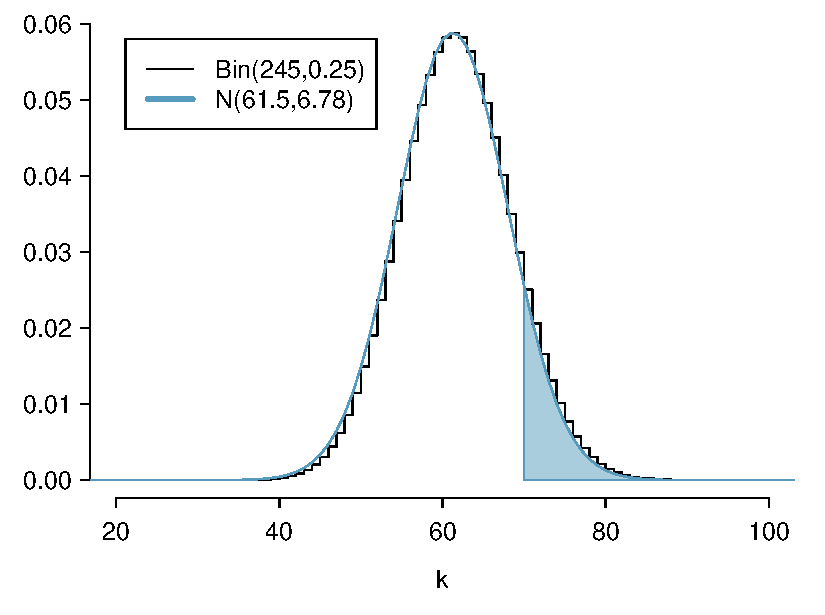
\includegraphics[width=0.5\textwidth]{3-4_binomial_distribution/figures/fb_power_user/fb_power_user}
\end{center}

\end{itemize}

\end{frame}

%%%%%%%%%%%%%%%%%%%%%%%%%%%%%%%%%%%

\begin{frame}
\frametitle{}

\dq{What is the probability that the average Facebook user with 245 friends has 70 or more friends who would be considered power users?}

\pause

\twocol{0.5}{0.5}{
\begin{center}
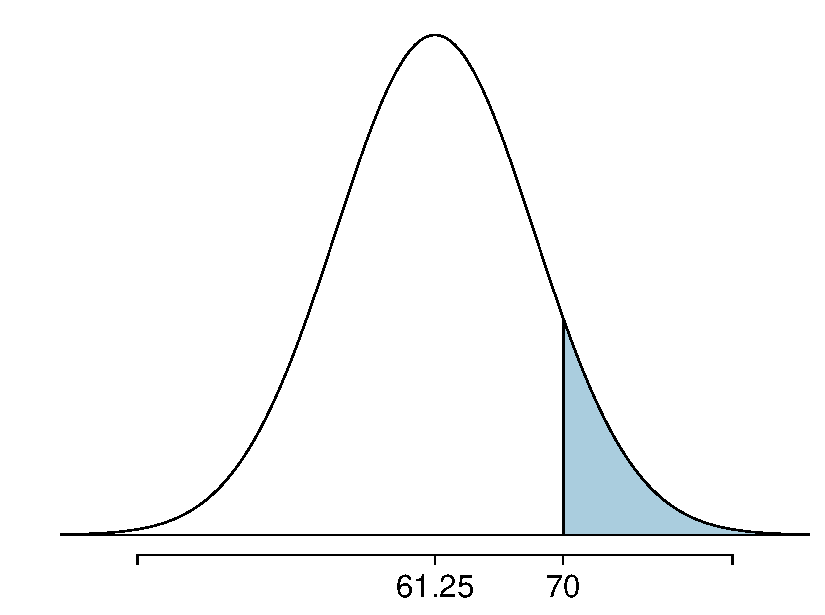
\includegraphics[width=\textwidth]{3-4_binomial_distribution/figures/fb_power_user/fb_power_user_norm}
\end{center}
}
{
\pause
\[ Z = \frac{obs - mean}{SD} = \frac{70 - 61.25}{6.78} = 1.29 \]

\pause
{\footnotesize
\begin{tabular}{c | rrrr>{\columncolor[gray]{0.6}[0pt]}r |}
  \cline{2-6}
& \multicolumn{5}{c}{Second decimal place of $Z$}  \\
  \cline{2-6}
$Z$ & 0.05 & 0.06 & 0.07 & 0.08 & 0.09   \\
  \hline
  \hline
  1.0 & \tiny{0.8531} & \tiny{0.8554} & \tiny{0.8577} & \tiny{0.8599} & \tiny{0.8621} \\
  1.1 & \tiny{0.8749} & \tiny{0.8770} & \tiny{0.8790} & \tiny{0.8810} & \tiny{0.8830} \\
\rowcolor[gray]{.6}
  1.2 & \tiny{0.8944} & \tiny{0.8962} & \tiny{0.8980} & \tiny{0.8997} & \red{\tiny{0.9015}} \\  
\end{tabular}
}

\pause
\[ P(Z > 1.29) = 1 - 0.9015 = 0.0985 \]
}

\end{frame}

%%%%%%%%%%%%%%%%%%%%%%%%%%%%%%%%%%


\end{document}
%%%%%%%%%%%%%%%%%%%%%%%%%%%%%%%%%%%%

\section{More discrete distributions}

%%%%%%%%%%%%%%%%%%%%%%%%%%%%%%%%%%%%

\subsection{Negative binomial distribution}

%%%%%%%%%%%%%%%%%%%%%%%%%%%%%%%%%%%%

\begin{frame}
\frametitle{Negative binomial distribution}

\begin{itemize}

\item The \hl{negative binomial distribution} describes the probability of observing the $k^{th}$ success on the $n^{th}$ trial.

\item The following four conditions are useful for identifying a negative binomial case:
\begin{enumerate}
\item The trials are independent.
\item Each trial outcome can be classified as a success or failure.
\item The probability of success ($p$) is the same for each trial.
\item The last trial must be a success.
\end{enumerate}
Note that the first three conditions are common to the binomial distribution.

\end{itemize}

\vfill

\formula{Negative binomial distribution}
{
P($k^{th}$ success on the $n^{th}$ trial) = ${n-1 \choose k-1}~p^k~(1-p)^{n-k}$, \\
where $p$ is the probability that an individual trial is a success. All trials are assumed to be independent.
}

\end{frame}

%%%%%%%%%%%%%%%%%%%%%%%%%%%%%%%%%%%%

\begin{frame}

\dq{A college student working at a psychology lab is asked to recruit 10 couples to participate in a study. She decides to stand outside the student center and ask every 5$^{th}$ person leaving the building whether they are in a relationship and, if so, whether they would like to participate in the study with their significant other. Suppose the probability of finding such a person is 10\%. What is the probability that she will need to ask 30 people before she hits her goal?}

\pause

Given: $p = 0.10$, $k = 10$, $n = 30$. We are asked to find the probability of $10^{th}$ success on the $30^{th}$ trial, therefore we use the negative binomial distribution.

\pause

\begin{eqnarray*}
P(\text{$10^{th}$ success on the $30^{th}$ trial}) &=& {29 \choose 9} \times 0.10^{10} \times 0.90^{20} \\
\pause
&=& 10,015,005 \times 0.10^{10} \times 0.90^{20} \\
\pause
&=& 0.00012
\end{eqnarray*}

\end{frame}

%%%%%%%%%%%%%%%%%%%%%%%%%%%%%%%%%%%%

\begin{frame}
\frametitle{Binomial vs. negative binomial}

\dq{How is the negative binomial distribution different from the binomial distribution?}

\pause

\begin{itemize}

\item In the binomial case, we typically have a fixed number of trials and instead consider the number of successes. 

\item In the negative binomial case, we examine how many trials it takes to observe a fixed number of successes and require that the last observation be a success.

\end{itemize}

\end{frame}

%%%%%%%%%%%%%%%%%%%%%%%%%%%%%%%%%%%%

\begin{frame}
\frametitle{Practice}

\pq{Which of the following describes a case where we would use the negative binomial distribution to calculate the desired probability?}

\begin{enumerate}[(a)]

\item Probability that a 5 year old boy is taller than 42 inches.

\item Probability that 3 out of 10 softball throws are successful.

\item Probability of being dealt a straight flush hand in poker.

\item Probability of missing 8 shots before the first hit.

\solnMult{Probability of hitting the ball for the 3${rd}$ time on the 8$^{th}$ try.}

\end{enumerate}

\end{frame}

%%%%%%%%%%%%%%%%%%%%%%%%%%%%%%%%%%%%

\subsection{Poisson distribution}

%%%%%%%%%%%%%%%%%%%%%%%%%%%%%%%%%%%%

\begin{frame}
\frametitle{Poisson distribution}

\begin{itemize}

\item The \hl{Poisson distribution} is often useful for estimating the number of rare events in a large population over a short unit of time for a fixed population if the individuals within the population are independent.

\item The \hl{rate} for a Poisson distribution is the average number of occurrences in a mostly-fixed population per unit of time, and is typically denoted by \mathhl{\lambda}.

\item Using the rate, we can describe the probability of observing exactly $k$ rare events in a single unit of time.

\end{itemize}

\vfill

\formula{Poisson distribution}
{
P(observe $k$ rare events) = $\frac{\lambda^k e^{-\lambda}}{k!}$, \\
where $k$ may take a value 0, 1, 2, and so on, and $k!$ represents $k$-factorial. The letter $e \approx 2.718$ is the base of the natural logarithm. \\

The mean and standard deviation of this distribution are $\lambda$ and $\sqrt{\lambda}$, respectively.
}

\end{frame}

%%%%%%%%%%%%%%%%%%%%%%%%%%%%%%%%%%%%

\begin{frame}

\dq{Suppose that in a rural region of a developing country electricity power failures occur following a Poisson distribution with an average of 2 failures every week. Calculate the probability that in a given week the electricity fails only once.}

\pause

Given $\lambda = 2$.

\pause

\begin{eqnarray*}
P(\text{only 1 failure in a week}) &=& \frac{2^1 \times e^{-2}}{1!} \\
\pause
&=& \frac{2 \times e^{-2}}{1} \\
\pause
&=& 0.27
\end{eqnarray*}

\end{frame}

%%%%%%%%%%%%%%%%%%%%%%%%%%%%%%%%%%%%

\begin{frame}

\dq{Suppose that in a rural region of a developing country electricity power failures occur following a Poisson distribution with an average of 2 failures every week. Calculate the probability that on a given \underline{day} the electricity fails three times.}

\pause

We are given the weekly failure rate, but to answer this question we need to first calculate the average rate of failure on a given day: $\lambda_{day} = \frac{2}{7} = 0.2857$. Note that we are assuming that the probability of power failure is the same on any day of the week, i.e. we assume independence.

\pause

\begin{eqnarray*}
P(\text{3 failures on a given day}) &=& \frac{0.2857^1 \times e^{-0.2857}}{3!} \\
\pause
&=& \frac{0.2857 \times e^{-0.2857}}{6} \\
\pause
&=& 0.0358
\end{eqnarray*}

\end{frame}

%%%%%%%%%%%%%%%%%%%%%%%%%%%%%%%%%%%%

\begin{frame}
\frametitle{Is it Poisson?}

\begin{itemize}

\item A random variable may follow a Poisson distribution if the event being considered is rare, the population is large, and the events occur independently of each other

\item However we can think of situations where the events are not really independent. For example, if we are interested in the probability of a certain number of weddings over one summer, we should take into consideration that weekends are more popular for weddings.

\item In this case, a Poisson model may sometimes still be reasonable if we allow it to have a different rate for different times; we could model the rate as higher on weekends than on weekdays.

\item The idea of modeling rates for a Poisson distribution against a second variable (day of the week) forms the
foundation of some more advanced methods called \hl{generalized linear models}. There are beyond the scope of this course, but we will discuss a foundation of linear models in Chapters 7 and 8.

\end{itemize}

\end{frame}

%%%%%%%%%%%%%%%%%%%%%%%%%%%%%%%%%%%%

\begin{frame}
\frametitle{Practice}

\pq{A random variable that follows which of the following distributions can take on values other than positive integers?}

\begin{enumerate}[(a)]
\item Poisson
\item Negative binomial
\item Binomial
\solnMult{Normal}
\item Geometric
\end{enumerate}

\end{frame}

%%%%%%%%%%%%%%%%%%%%%%%%%%%%%%%%%%%%

\end{document}

%%%%%%%%%%%%%%%%%%%%%%%%%%%%%%%%%%%%

\end{document}